%%%%%%%%%%%%%%%%%%%%%%%% ADD CONTENT %%%%%%%%%%%%%%%%%%%%%%

\section{Analysis and plotting of spatial data}

\begin{frame}
   \vspace{1.5cm}
   From file .....   \\
   \vspace{1.5cm}
   \hspace{5cm}  to figure ...  \\
\end{frame}

%*****************************************************************
% SEC0 | Outline
%*****************************************************************
\begin{frame}{\textbf{0 |}Outline}
   Outline:
   \begin{itemize}
       \item Downloaded a file, so what?
            \vspace{0.3cm}
       \item Play around with CDO
            \vspace{0.3cm}
       \item Load into Python and visualise
            \vspace{0.3cm}
       \item Make a publication figure
   \end{itemize}
\end{frame}

%*****************************************************************
% SEC1 | Downloaded a file, so what?
%*****************************************************************
\begin{frame}{\textbf{1 |} Downloaded a file, so what?}
Using \textbf{ncview} to check the file:
   \begin{itemize}
       \item Dimensions? right domain?
            \vspace{0.3cm}
       \item Variables?
            \vspace{0.3cm}
       \item Units? and Range?
            \vspace{0.3cm}
       \item Quick check for Mask
            \vspace{0.3cm}
       \item Timeseries
   \end{itemize}
\end{frame}


\begin{frame}{\textbf{1 |} Downloaded a file, so what?}
    Using  \textbf{ncview} to check the file:
    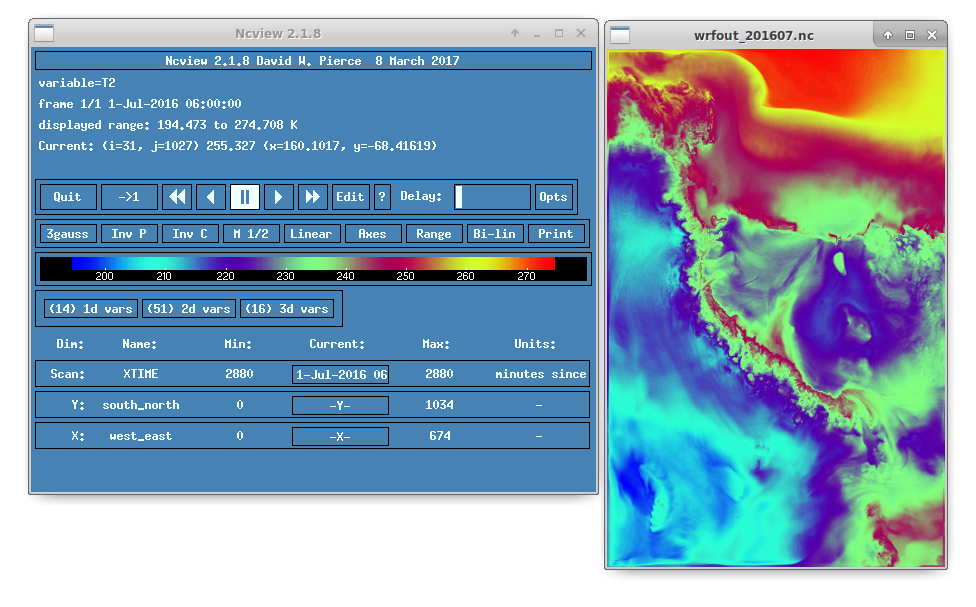
\includegraphics[scale=0.3]{images/wrf_RIS.png}\\
        \centering\tiny{WRF output, 2m temperature}
\end{frame}


\begin{frame}{\textbf{1 |} Downloaded a file, so what?}
    Using \textbf{ncview} to check the file:
    \begin{columns}
        \column[c]{6.5cm}
            \centering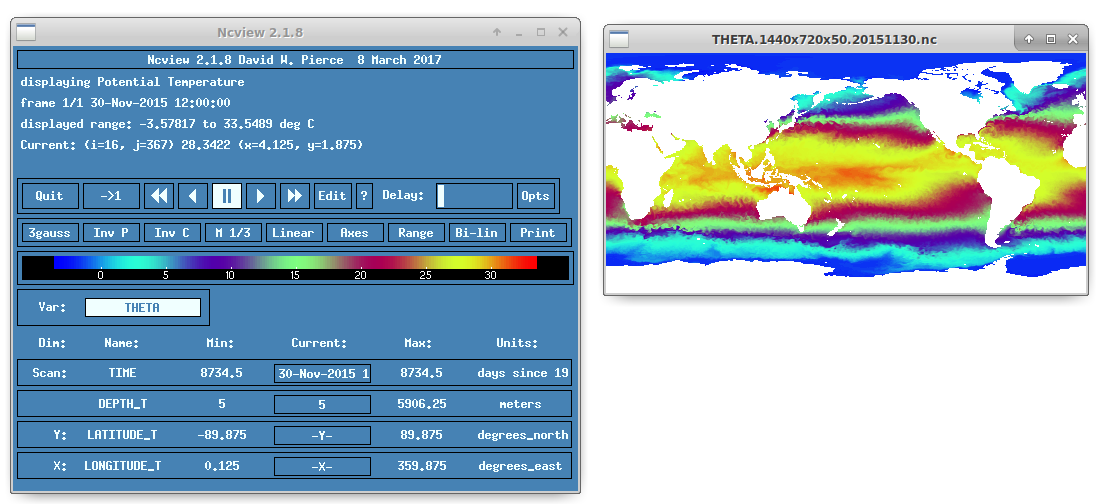
\includegraphics[width=6cm]{images/Theta.png} \\
                \centering\tiny{ECCO2, potential temperature}
        \column[c]{6.5cm}
    \end{columns}
\end{frame}


\begin{frame}{\textbf{1 |} Downloaded a file, so what?}
    Using \textbf{ncview} to check the file:
    \begin{columns}
        \column[c]{6.5cm}
            \centering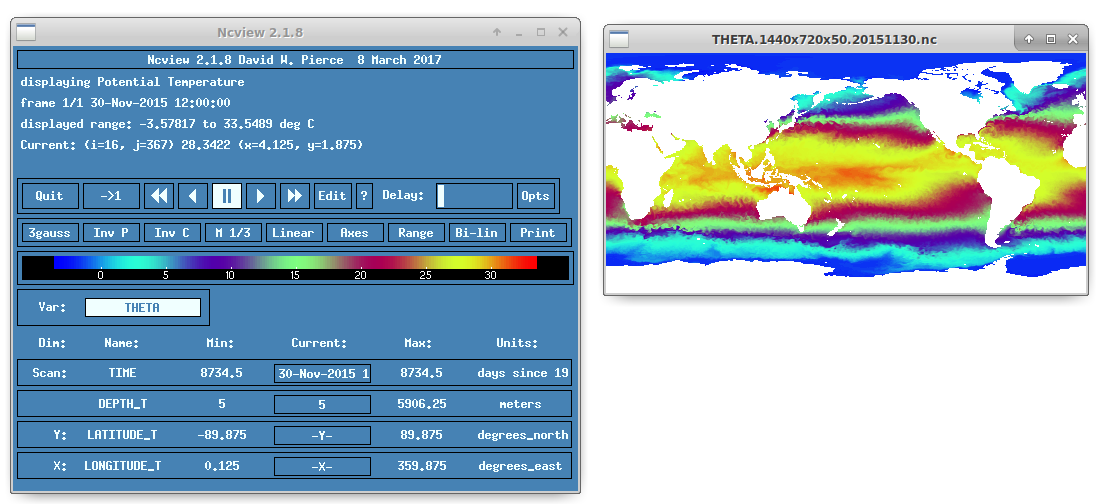
\includegraphics[width=6cm]{images/Theta.png} \\
                \centering\tiny{ECCO2, potential temperature}
        \column[c]{6.5cm}
            \centering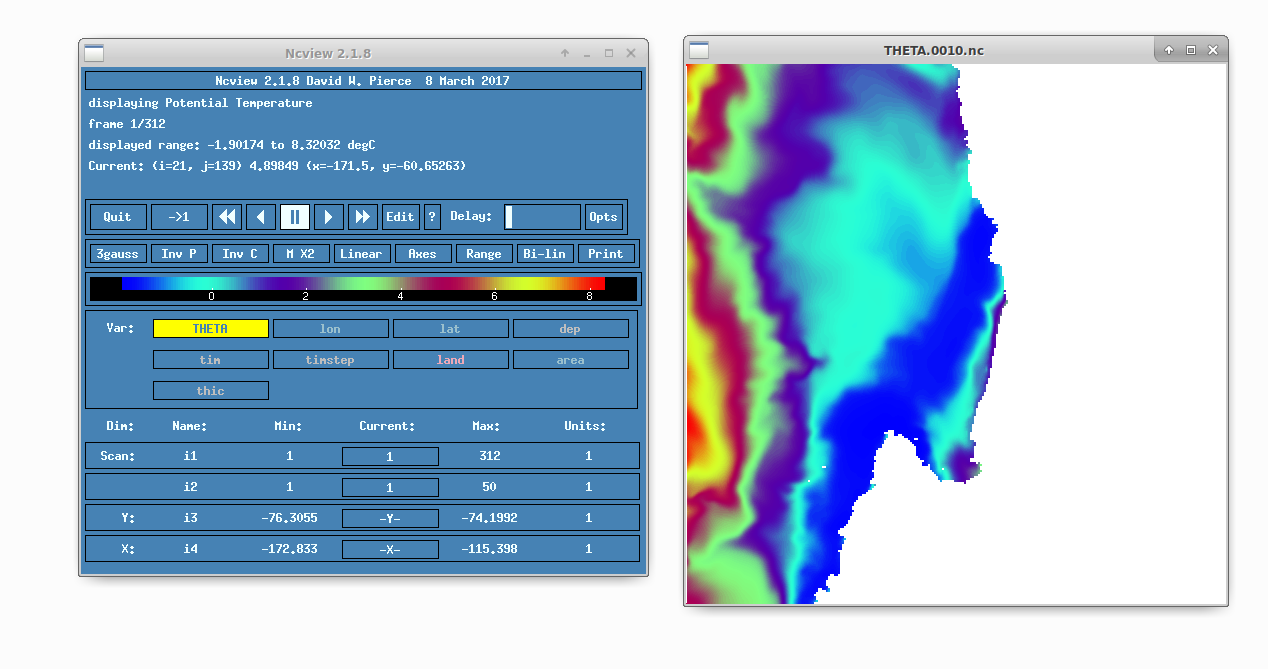
\includegraphics[width=6cm]{images/MIT_eccoV5.png} \\
                \centering\tiny{ECCO v5, potential temperature}
    \end{columns}
\end{frame}
ausgust 

\begin{frame}{\textbf{1 |} Downloaded a file, so what?}
    Using \textbf{ncview} to check the file:
    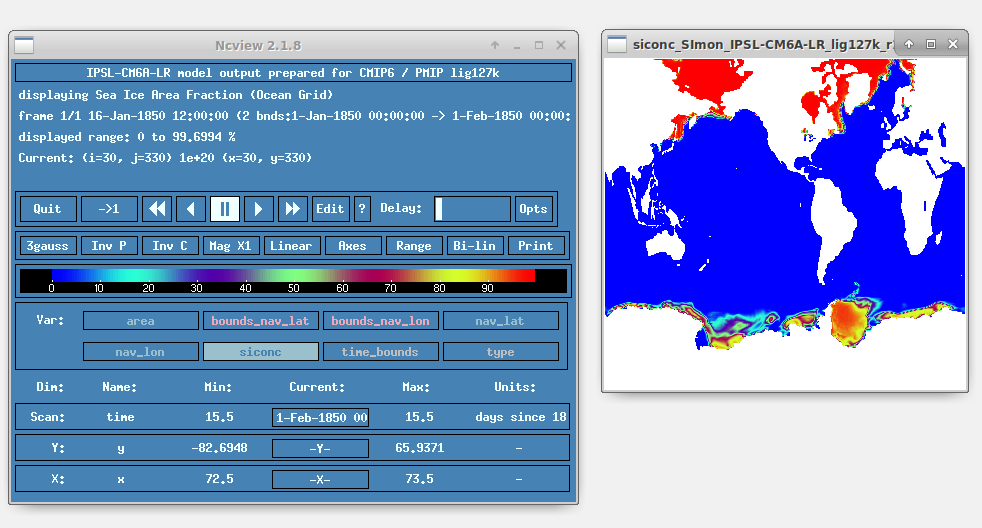
\includegraphics[scale=0.3]{images/tripolar.png}
        \centering\tiny{IPSL-CM6A-LR, sea ice area fraction}
\end{frame}


\begin{frame}{\textbf{1 |} Downloaded a file, so what?}
    Using \textbf{panoply} to check the file:
    \centering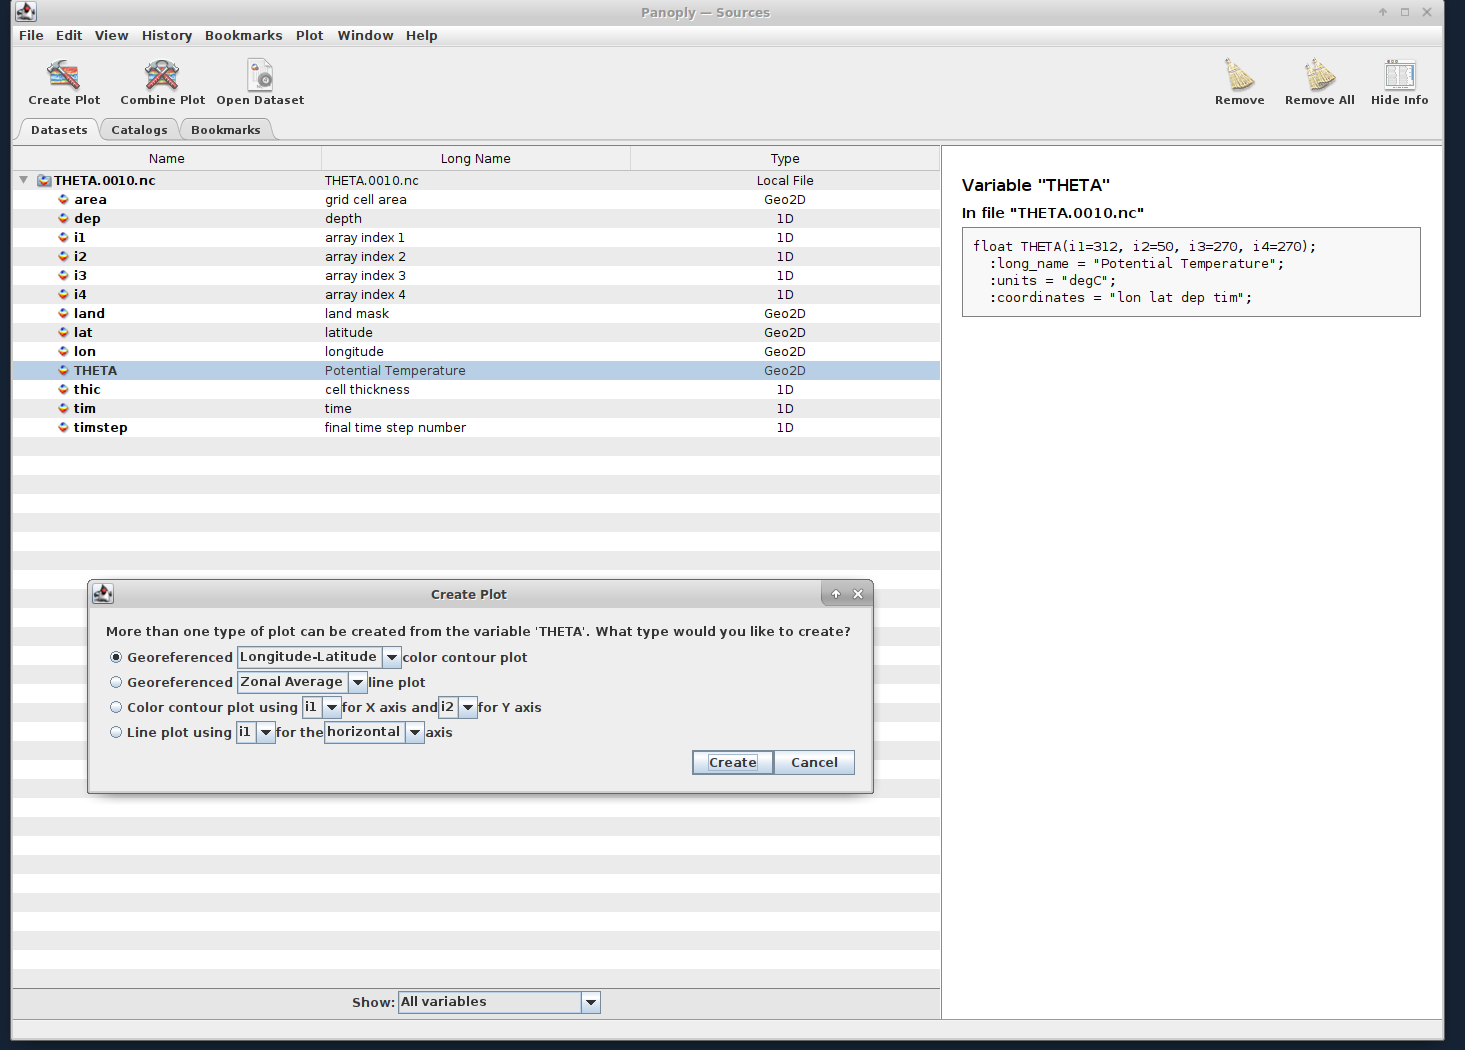
\includegraphics[width=10cm]{images/Panoply1.png} \\
\end{frame}


\begin{frame}{\textbf{1 |} Downloaded a file, so what?}
    Using \textbf{panoply} to check the file:
    \centering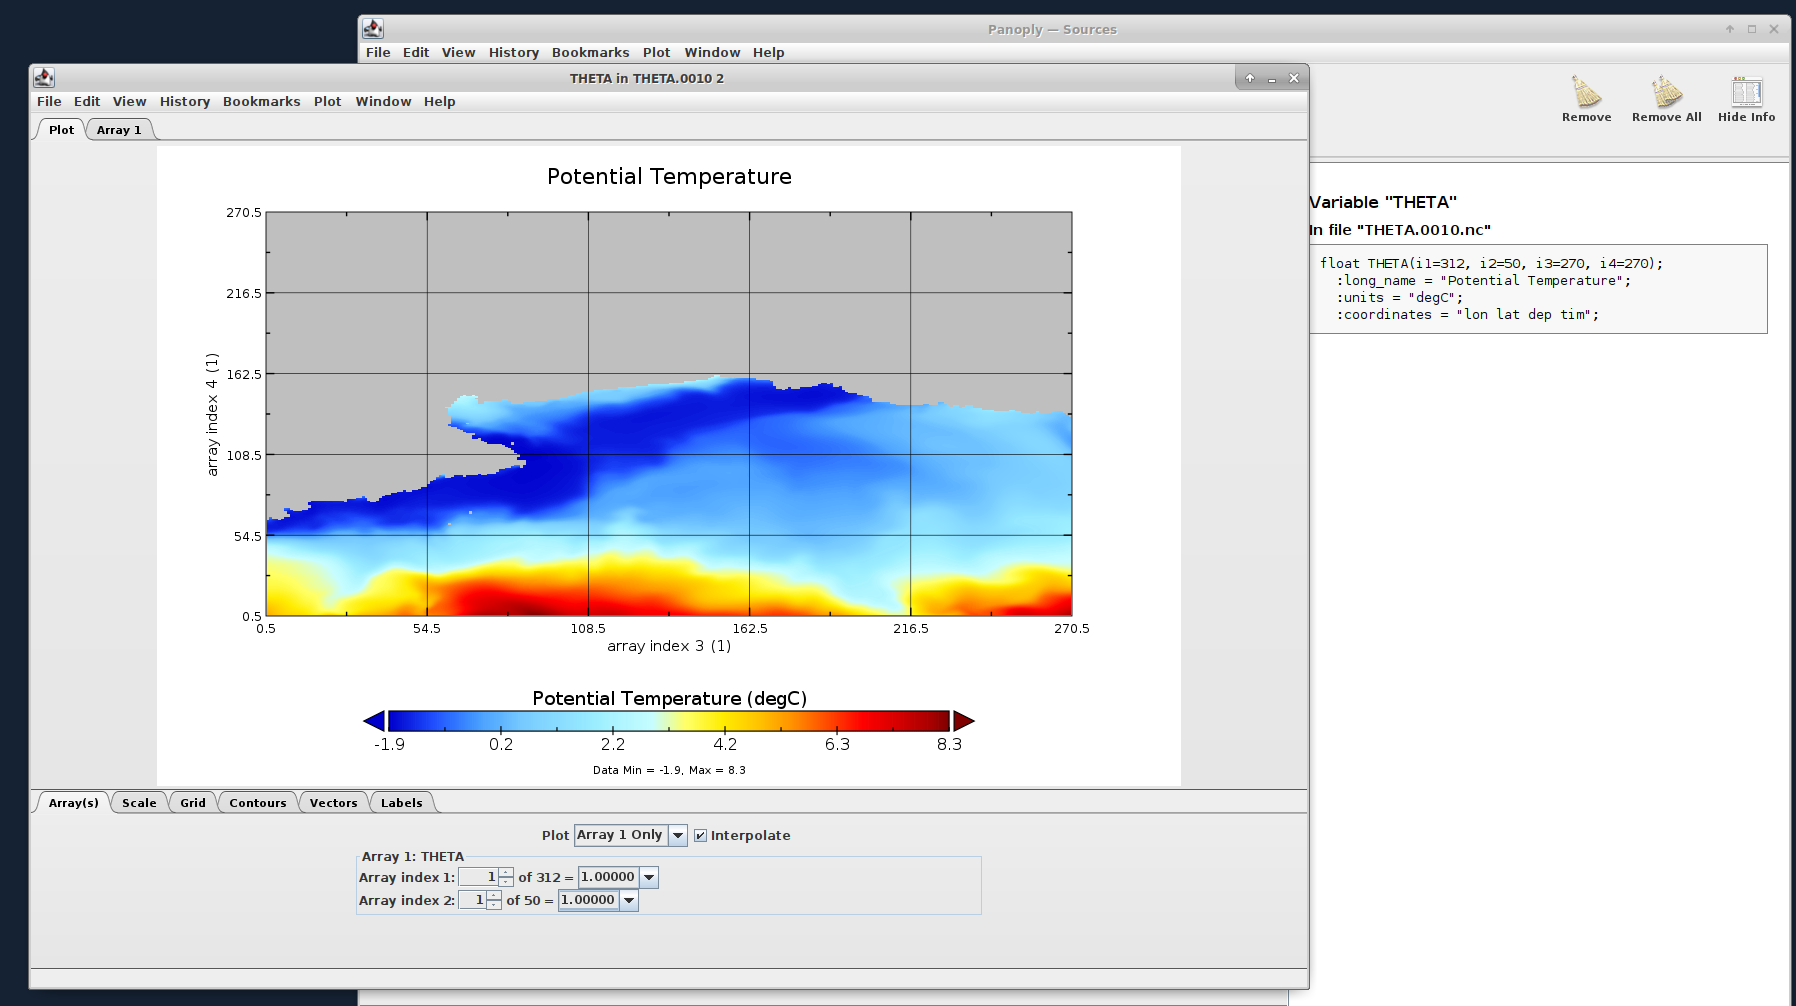
\includegraphics[width=10cm]{images/Panoply2.png} \\
\end{frame}


\begin{frame}{\textbf{1 |} Downloaded a file, so what?}
    Using \textbf{panoply} to check the file:
    \centering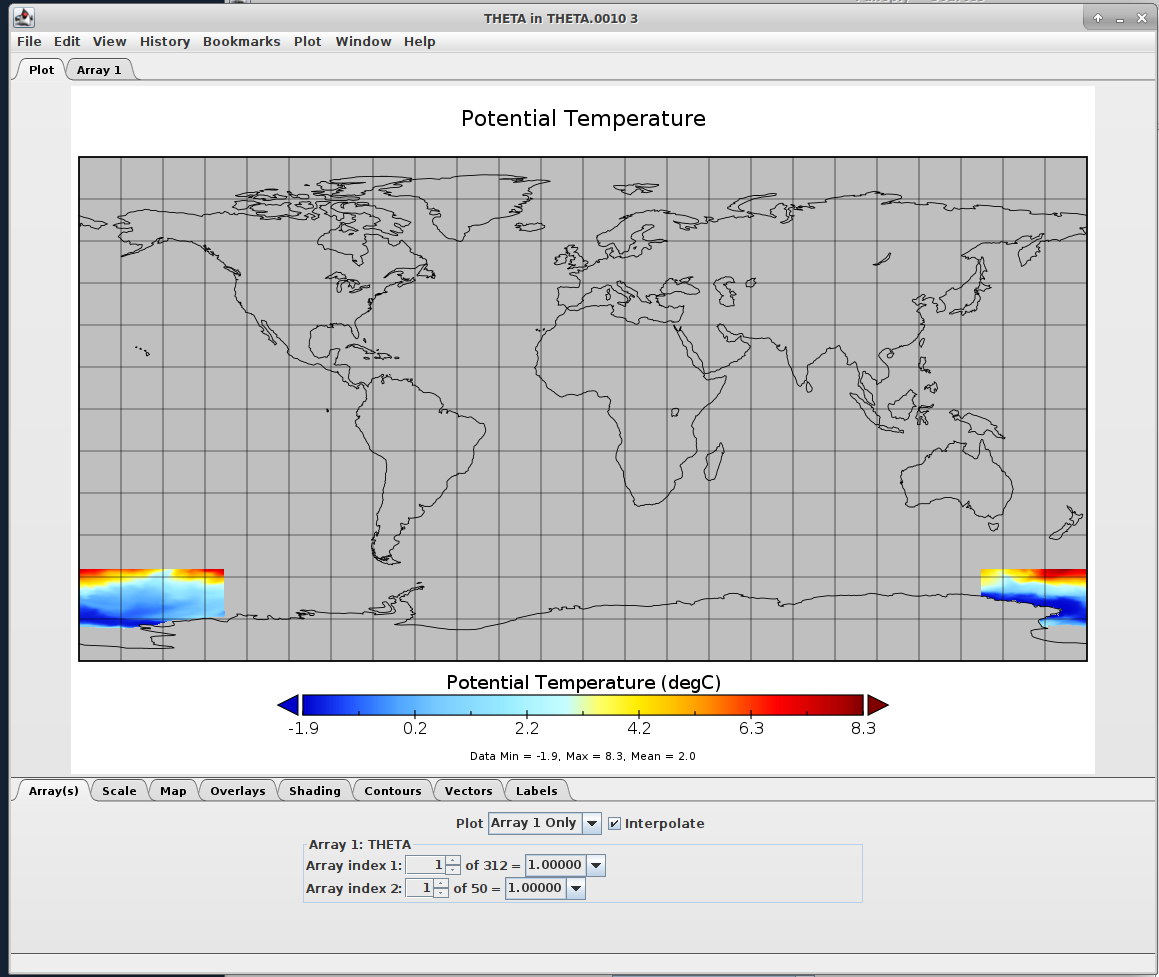
\includegraphics[width=8.5cm]{images/Panoply3.png} \\
\end{frame}


\begin{frame}{\textbf{1 |} Downloaded a file, so what?}
    Using \textbf{panoply} to check the file:
    \centering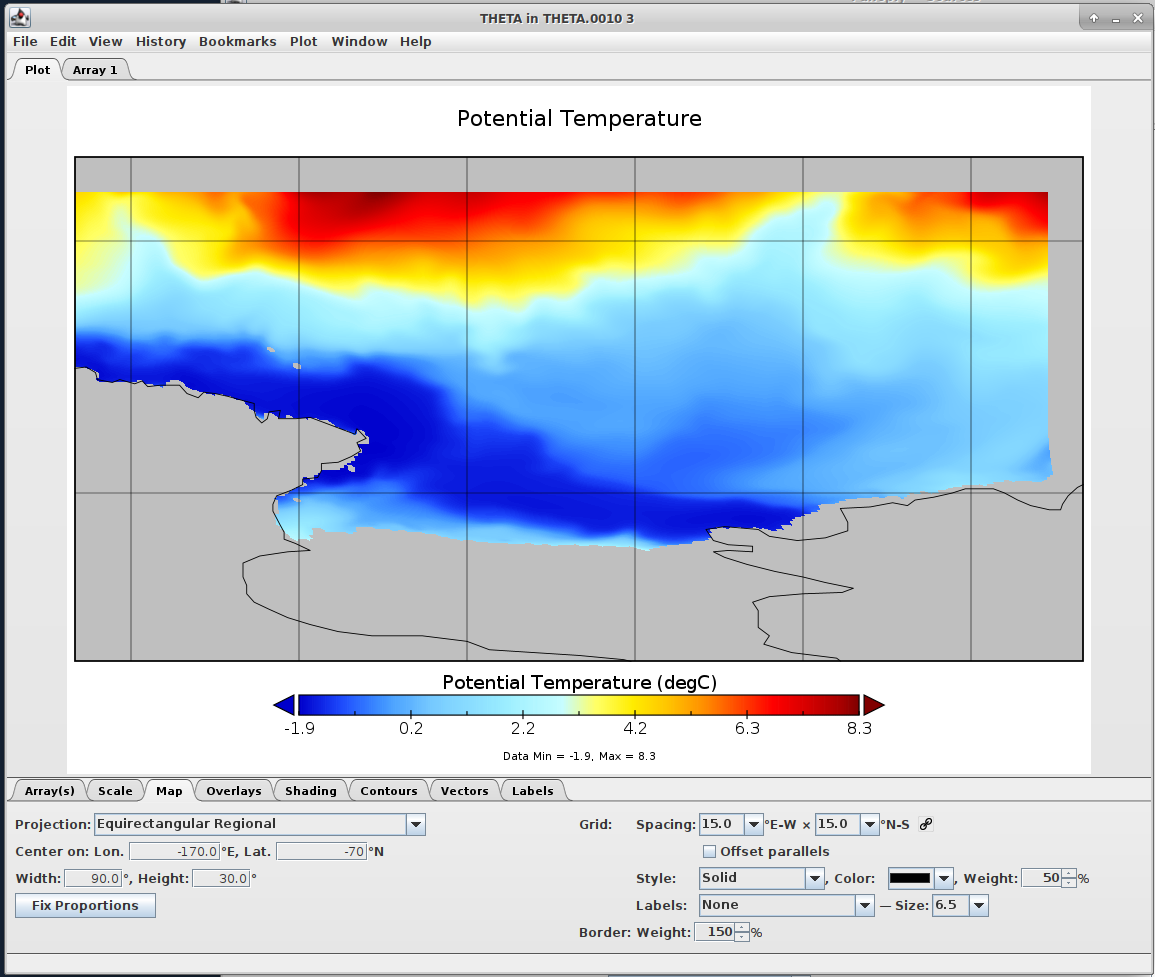
\includegraphics[width=8.5cm]{images/Panoply4.png} \\
\end{frame}


\begin{frame}{\textbf{1 |} Downloaded a file, so what?}
    Using \textbf{panoply} to check the file:
    \centering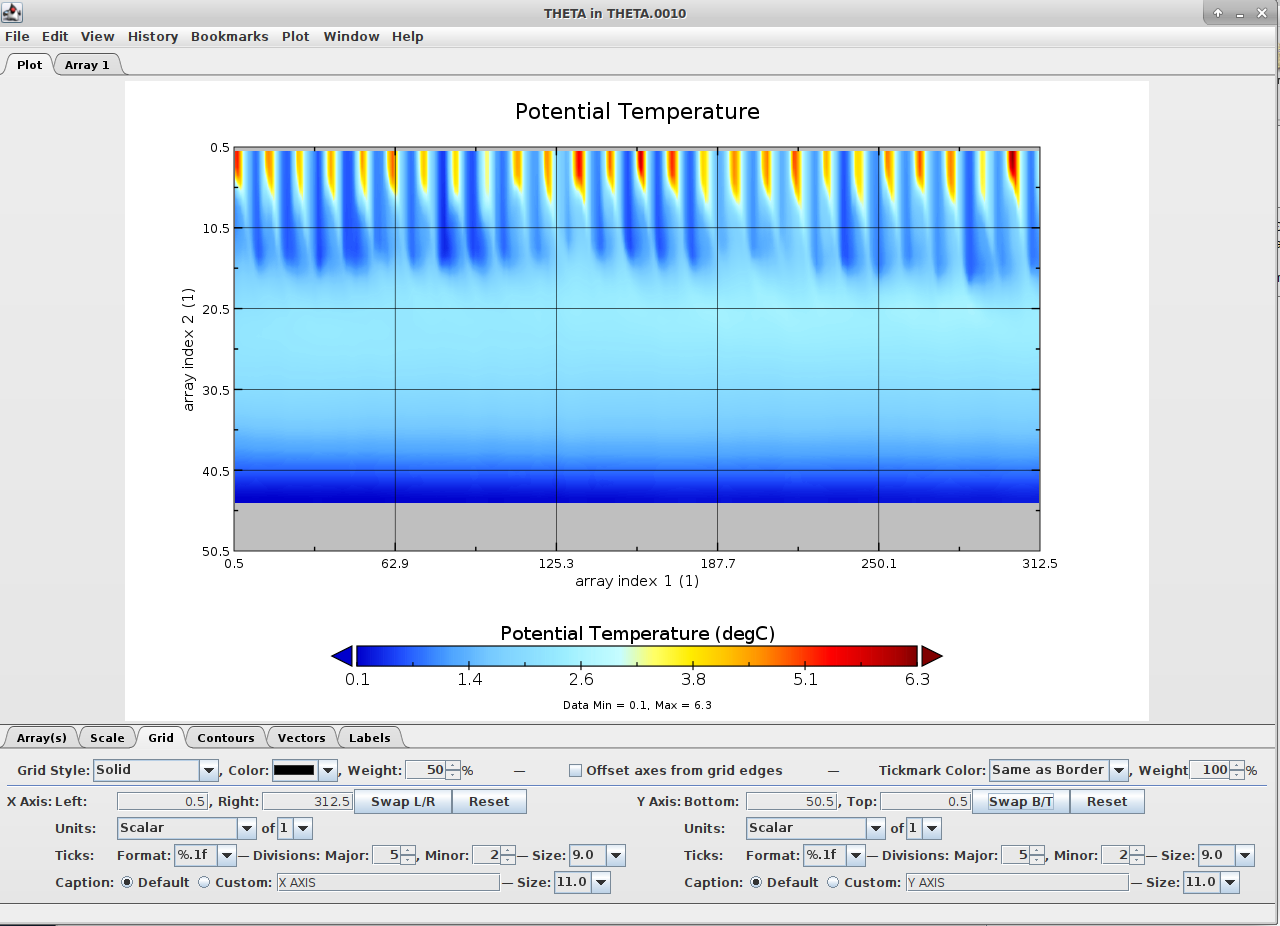
\includegraphics[width=10cm]{images/Panoply5.png} \\
\end{frame}


\begin{frame}{\textbf{1 |} Downloaded a file, so what?}
    Using \textbf{panoply} to check the file:
    \centering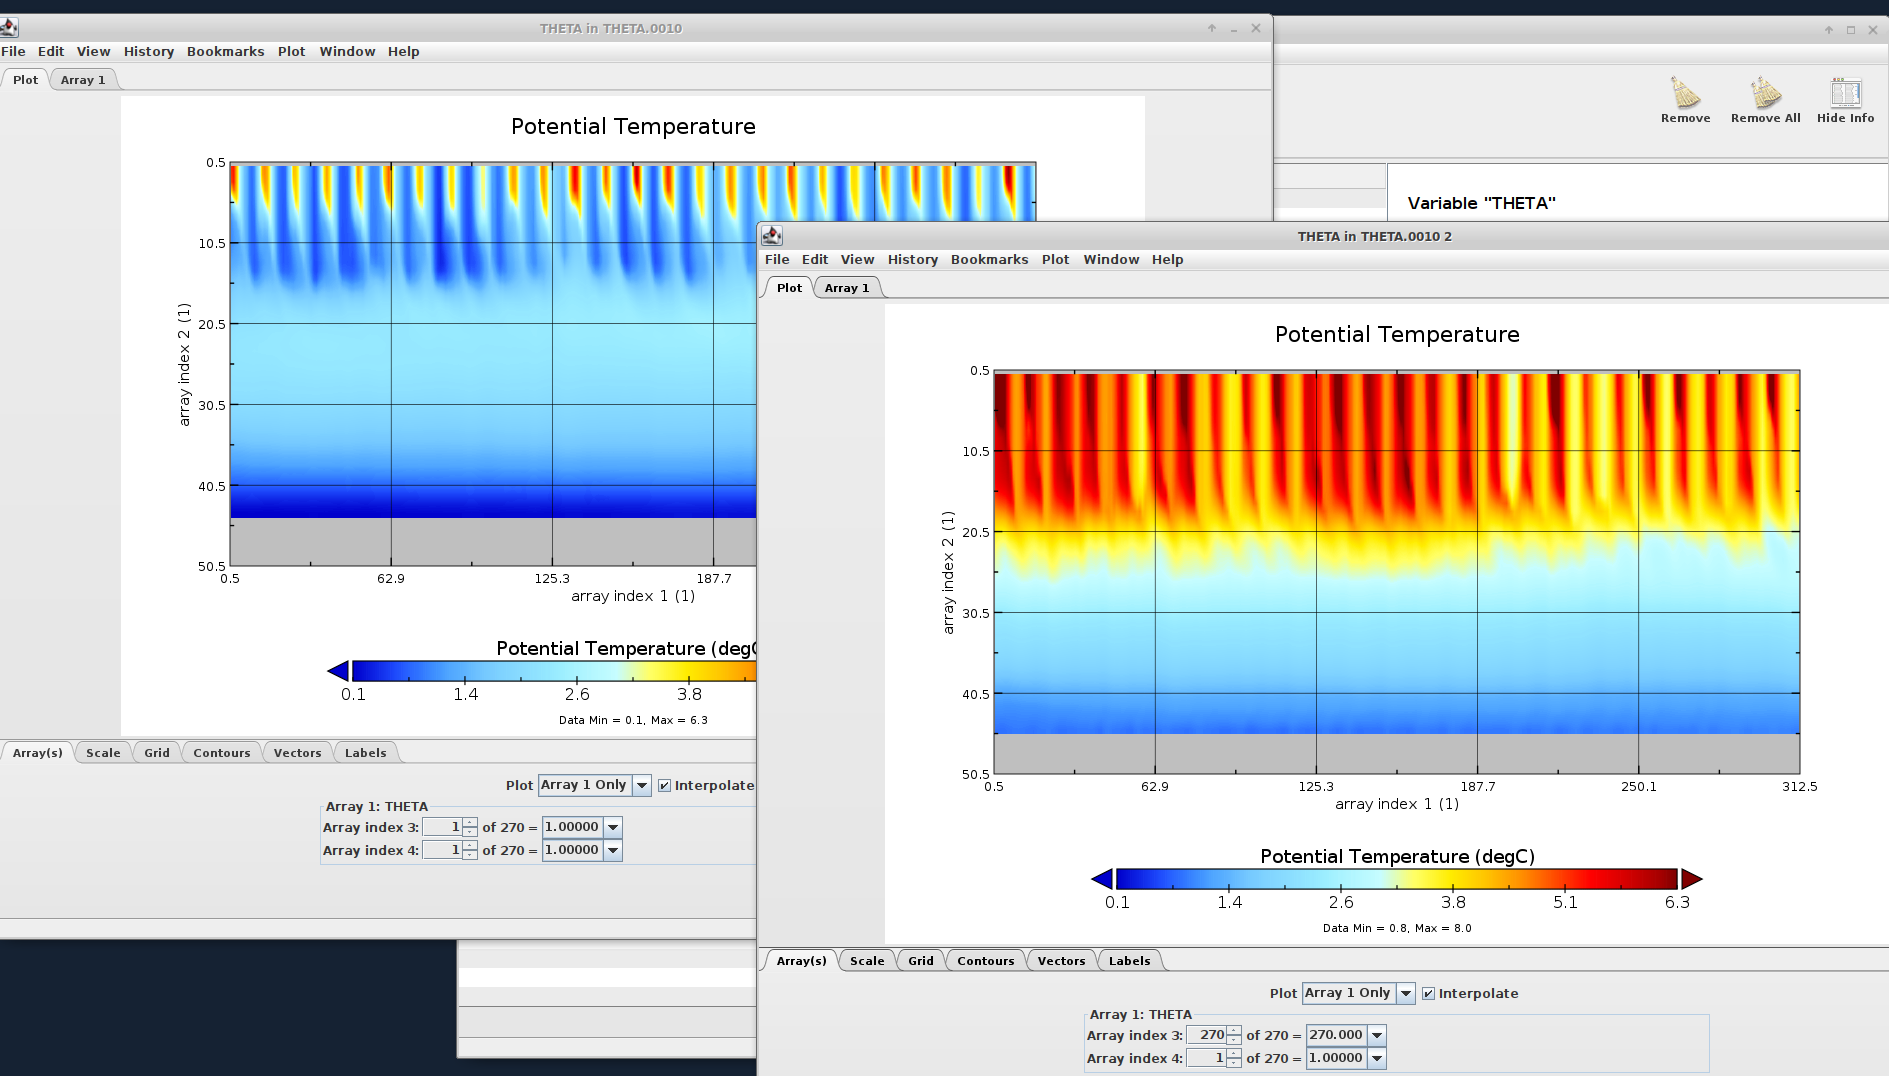
\includegraphics[width=10cm]{images/Panoply6.png} \\
\end{frame}


\begin{frame}{\textbf{1 |} Downloaded a file, so what?}
    Using \textbf{panoply} to check the file:
    \centering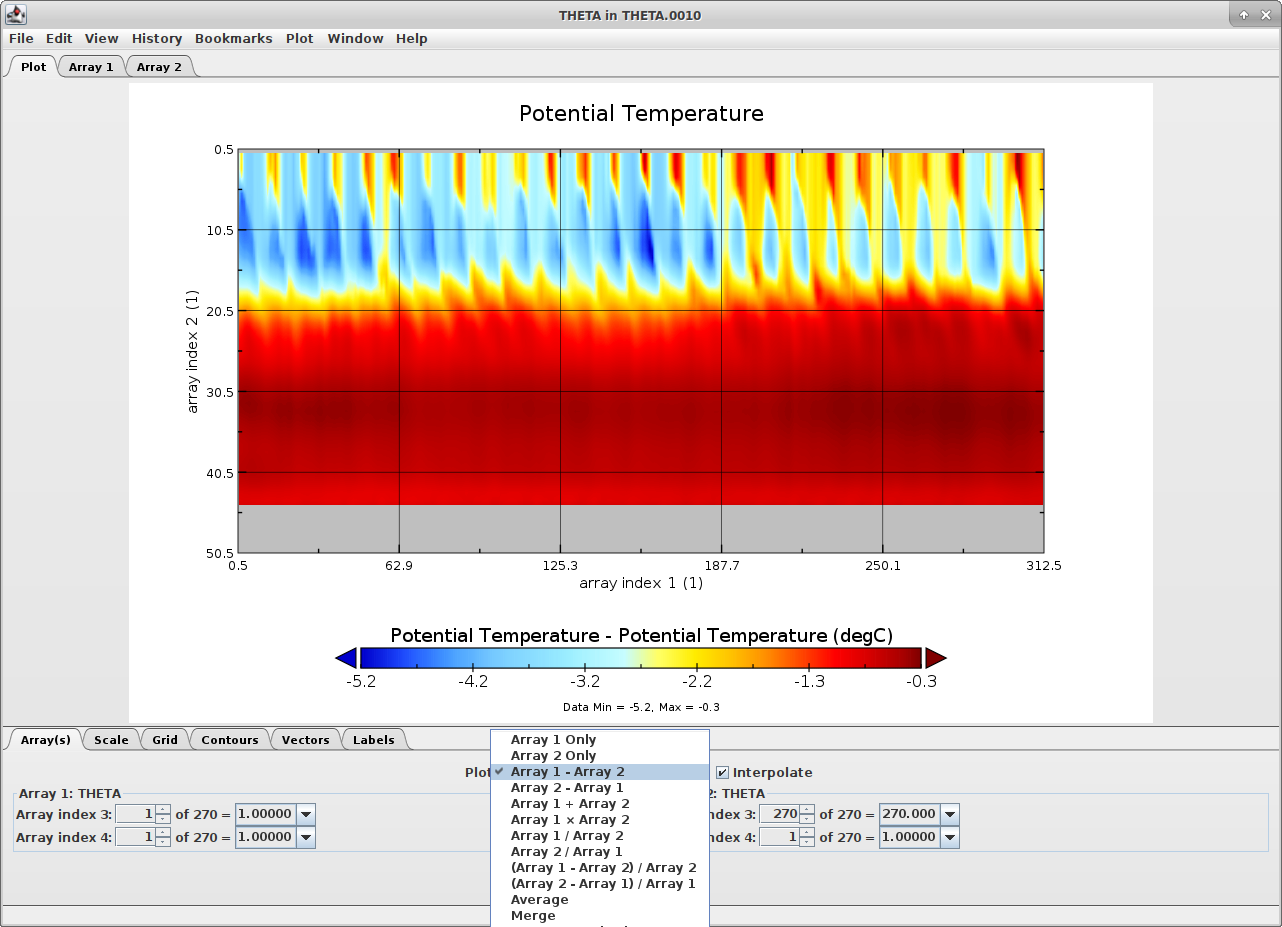
\includegraphics[width=10cm]{images/Panoply7.png} \\
\end{frame}


\begin{frame}{\textbf{1 |} Downloaded a file, so what?}
    Using \textbf{panoply} to check the file:
    \centering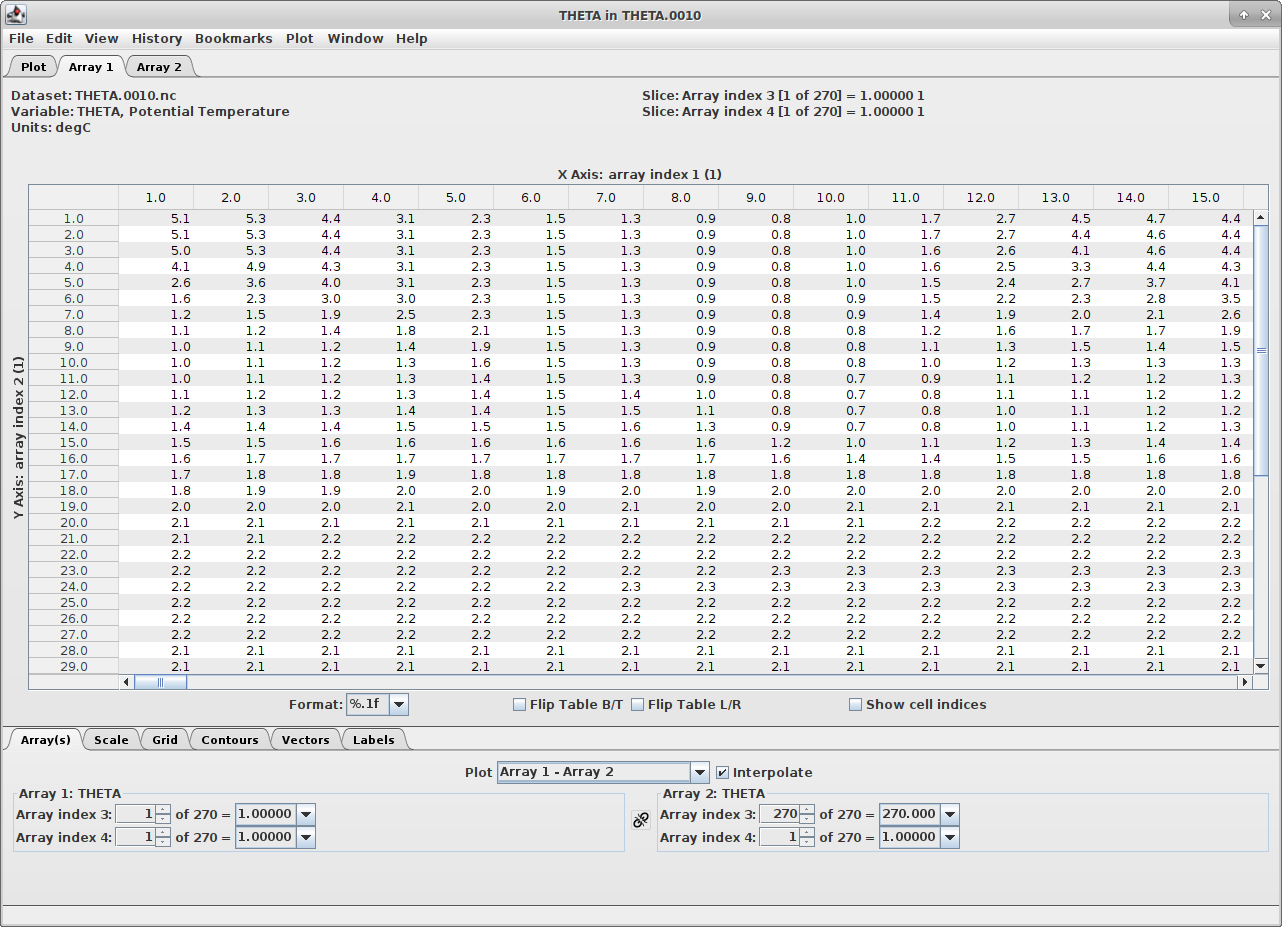
\includegraphics[width=10cm]{images/Panoply8.png} \\
\end{frame}


\begin{frame}{\textbf{1 |} Downloaded a file, so what?}
    Different coordinate systems:
        \vspace{0.3cm}
    \begin{itemize}
        \item lon-lat (easy to figure out where we are)
            \vspace{0.3cm}
        \item x-y (equidistant grid in km, better at the poles)
            \vspace{0.3cm}
        \item irregular grid (removes the pole problem)
    \end{itemize}
\end{frame}


\begin{frame}{\textbf{1 |} Downloaded a file, so what?}
    Different coordinate systems:
    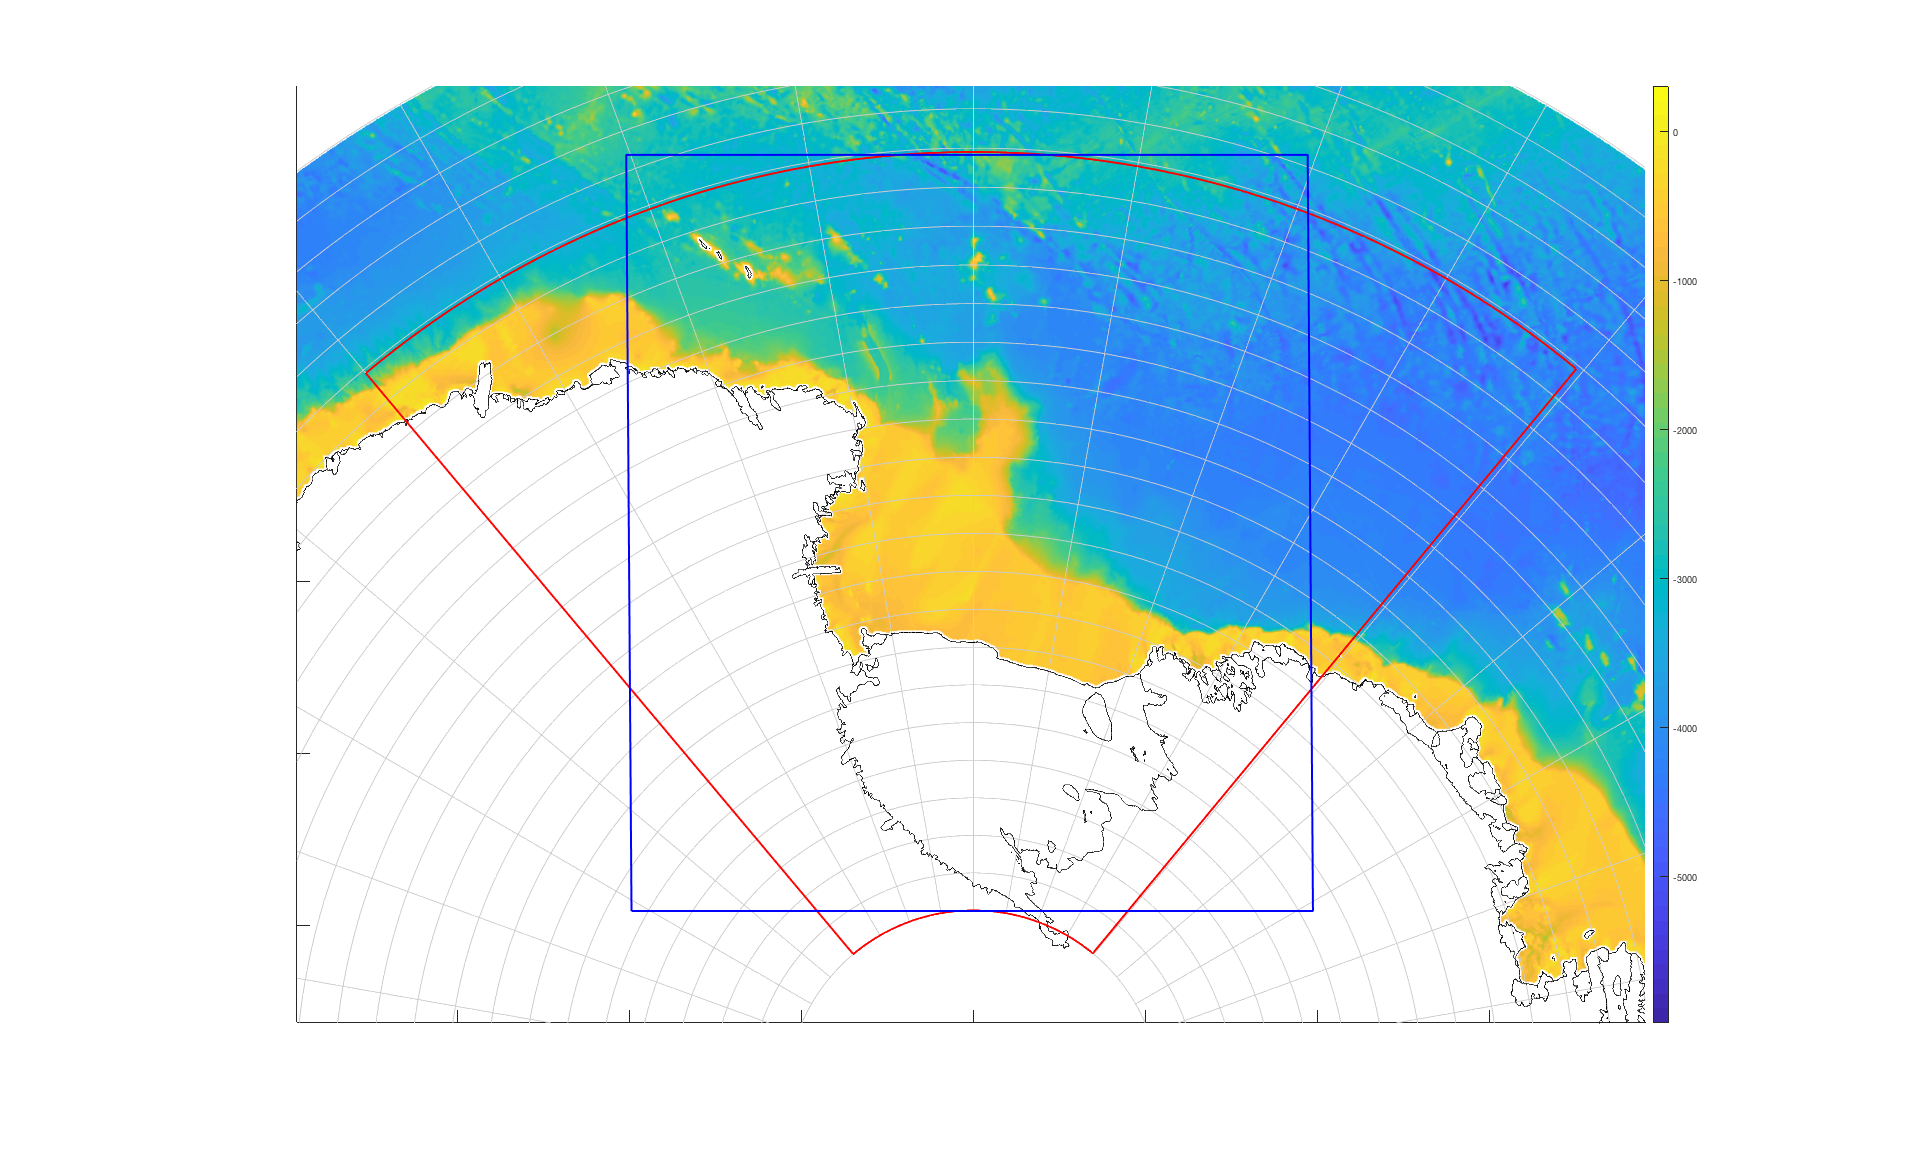
\includegraphics[scale=0.15]{images/winter_school_domain_1.png}
\end{frame}


\begin{frame}{\textbf{1 |} Downloaded a file, so what?}
    Different coordinate systems:
    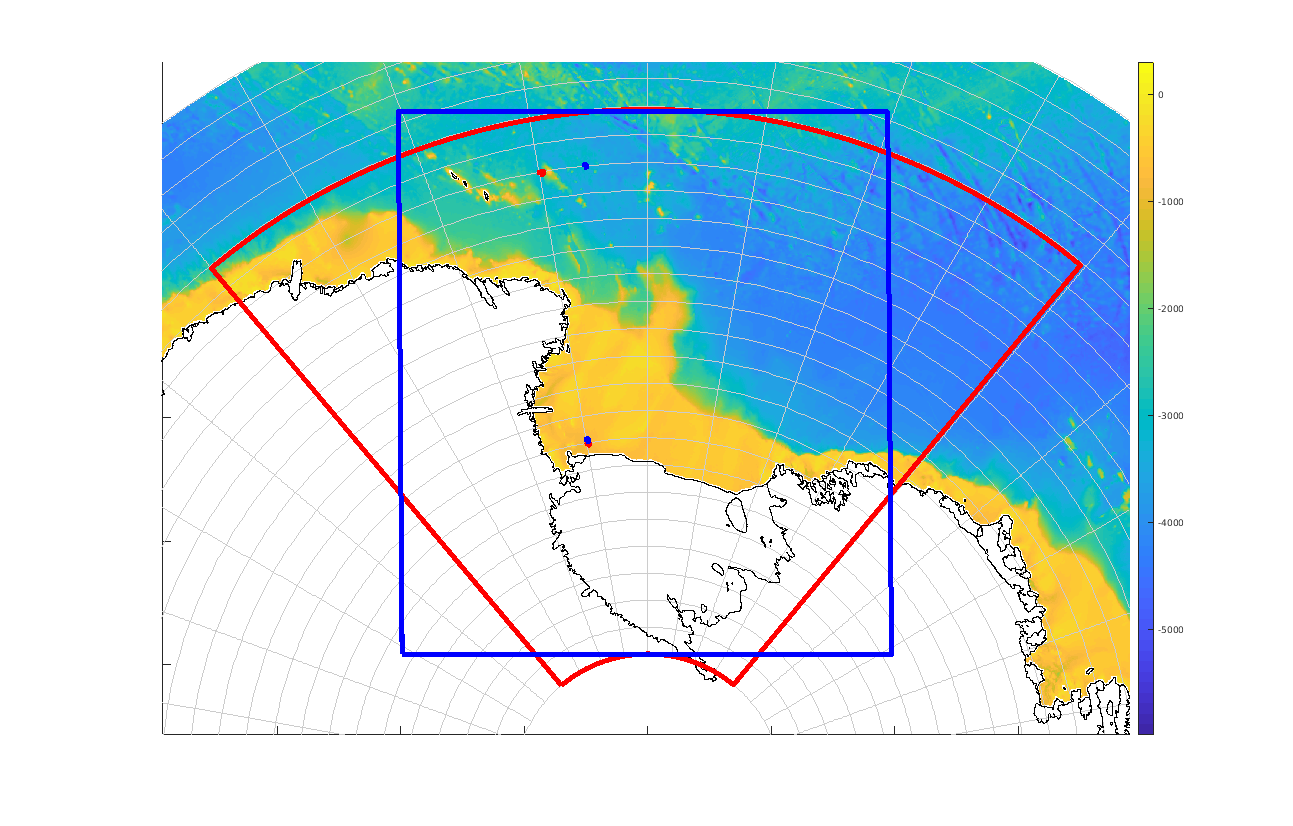
\includegraphics[scale=0.15]{images/winter_school_domain_2.png}
\end{frame}


\begin{frame}{\textbf{1 |} Downloaded a file, so what?}
    Different coordinate systems:
    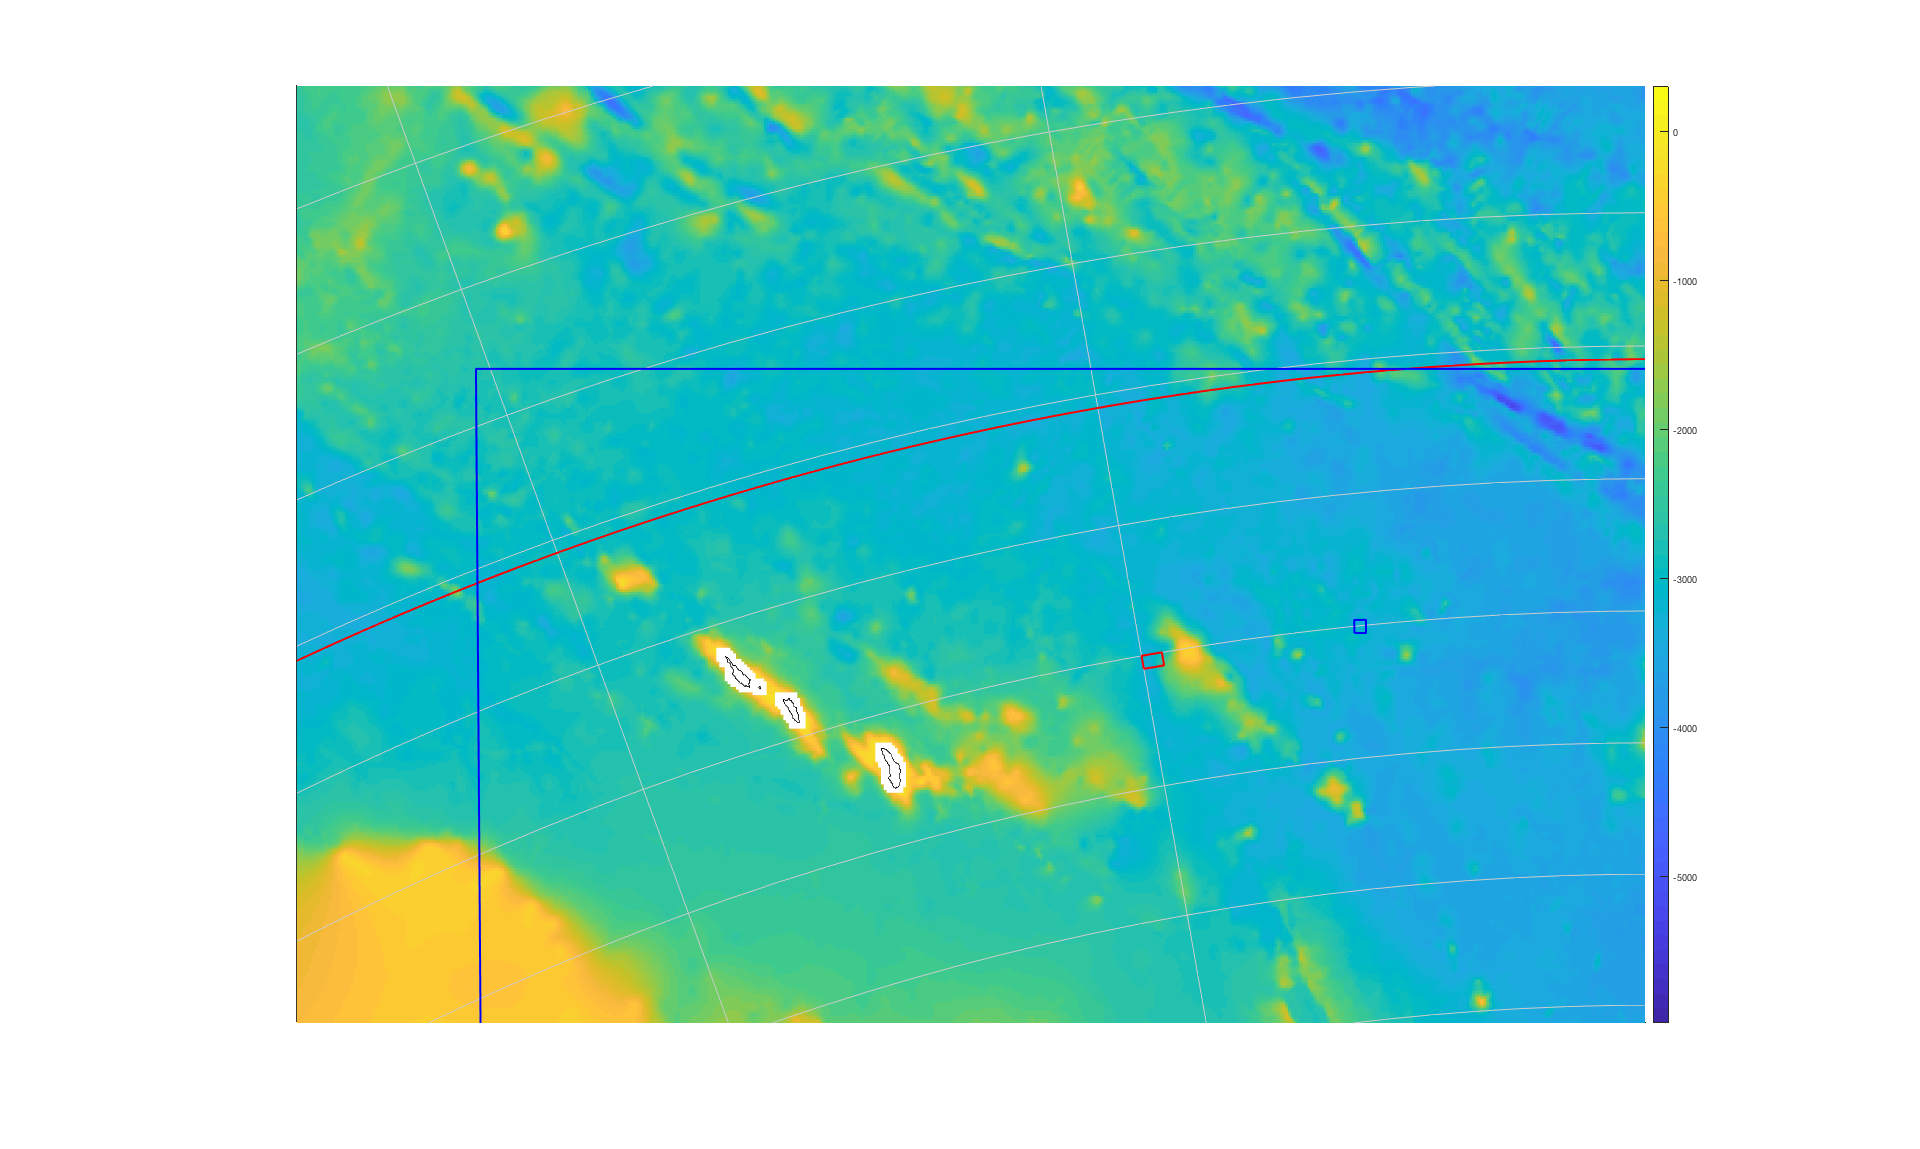
\includegraphics[scale=0.15]{images/winter_school_domain_3.png}
\end{frame}


\begin{frame}{\textbf{1 |} Downloaded a file, so what?}
    We can use ncview directly \\
        \begin{itemize}
            \item \textit{ncdump filename} 
            \item \textit{ncdump -h filename} 
            \item \textit{cdo sinfo filename} 
        \end{itemize}
    \vspace{2cm}
    \begin{beamerboxesrounded}[lower=gray,shadow=true]{Pop quiz: open the theta....2013.nc file and:
        \begin{itemize}
            \item what is the variable(s)? short and long name?
            \item what is the spatial resolution of the data? and the dimension of the file?
            \item what is the temporal coverage of the data?
         \item is there a mask value anywhere? 
         \item how many dimensions does this variable have?
        \end{itemize}
        }
    \end{beamerboxesrounded}
\end{frame}
 
 
%*****************************************************************
% SEC2 | Play around with CDO
%*****************************************************************

\begin{frame}{\textbf{2 |} Play around with \textbf{cdo}}
    Big files \textbf{WILL} make your matlab or python crash!\\
        \vspace{0.3cm}
    Pre-processing can save our life: let's use \href{http://www.idris.fr/media/ada/cdo.pdf}{\beamerbutton{CDO}}\\
        \vspace{0.5cm}
    to reduce the spatial extent:
    \begin{itemize}
        \item \textit{cdo sellonlatbox,lon0,lon1,lat0,lat1 infile outfile }
           \vspace{0.3cm}
        \item \textit{cdo selindexbox,index0,index1,index0,index1 infile outfile }
    \end{itemize}
        \vspace{0.4cm}
    example: to select New Zealand \\
        \vspace{0.3cm}
    \textcolor{black}{cdo sellonlatbox,150,180,-30,-50 thetao\_Omon\_CESM2\_historical\_r1i1p1f1\_gr\_201301-201412.nc NZ\_theta.nc }\\
        \vspace{0.3cm}
    and the same for salinity
\end{frame}
  
  
\begin{frame}{\textbf{2 |} Play around with CDO} 
    to reduce the temporal extent:
        \vspace{0.3cm}
    \begin{itemize} 
        \item \textit{cdo selmon,1 infile outfile }
            \vspace{0.3cm}
        \item \textit{cdo select,timestep=1  infile outfile }
            \vspace{0.3cm}
         \item \textit{cdo splityear  infile prefix- }
    \end{itemize}
\end{frame}


\begin{frame}{\textbf{2 |} Play around with CDO}
    to reduce the number of levels extent:\\
        \vspace{0.3cm}
    \textit{cdo sellevel,1 infile outfile }\\
        \vspace{0.3cm}
    \textit{cdo select,levrange=lev1,lev2,name=varname}\\
        \vspace{0.5cm}
    example: to select the second and third levels\\
        \vspace{0.5cm}
    \textcolor{black}{cdo select,level=10,20,name=thetao NZ\_theta.nc NZ\_theta\_levels.nc}\\
  \vspace{0.3cm}
        and do the same for salinity
\end{frame}


 \begin{frame}{\textbf{2 |} Play around with CDO} 
    But also to mask data, regrid and even do some stats ...\\
        \vspace{0.5cm}
    \begin{itemize}
        \item\textit{cdo ifthenelse ...} will use a condition to determine if the mask is used (! create a mask file beforehand) \\
                \vspace{0.3cm}
            example: Masking out the areas with salinity > 34.5 for the temperature file\\
                \vspace{0.3cm}
            \textcolor{black}{cdo mulc,0 NZ\_theta\_levels.nc zeroes.nc \\
            cdo ifthenelse -gec,34.5 NZ\_tso\_levels.nc zeroes.nc NZ\_theta\_levels.nc  test.nc}\\
                \vspace{0.5cm}
        \item\textit{cdo remapbil ...} will use bilinear interpolation to remap one grid ont another (! create a grid description file using \textit{cdo griddes} beforehand)\\
            \vspace{0.5cm}
        \item \textit{cdo monmean ...}, \textit{cdo ymonmean ...}, \textit{cdo add(c) ...}, \textit{cdo sub(c) ...}, \textit{cdo monstd ...}
    \end{itemize}
\end{frame}


 \begin{frame}{\textbf{2 |} Play around with CDO} 
    \begin{beamerboxesrounded}[lower=gray,shadow=true]{Pop quiz: Use \textbf{cdo} commands to         compare two cross sections of the mean June sst value over the dateline. \\
            \vspace{0.5cm}
        using the two thetao files (201301-201412 and 185001-185112).\\
            \vspace{0.5cm}
        and using the red-blue colormap, invert the y scale and make the colorbar symmetrical around 0\\
            \vspace{2cm}
        Hint: subtract one from the other}
    \end{beamerboxesrounded}
\end{frame}


%*****************************************************************
% SEC3 | Load into Python and visualise
%*****************************************************************

\begin{frame}{\textbf{3 |} Load into Python and visualise} 
    Now, time to create a script to make reproducible plots:
        \vspace{0.3cm}
    \begin{itemize}
        \item create a python script (decide\_on\_a\_relevant\_and\_clear\_name\textbf{.py})
             \vspace{0.3cm}
         \item one figure per file is a useful rule
             \vspace{0.3cm}
        \item add comments to explain what you do
             \vspace{0.3cm}
        \item prepare your data before loading it
             \vspace{0.3cm}
        \item tp run a python script : \textit{python scriptname.py} in the terminal
            \vspace{0.3cm}
    \end{itemize}
\end{frame}
 
 
 \begin{frame}{\textbf{3 |} Load into Python and visualise} 
    Let's import the relevant python packages:\\
        \vspace{0.3cm}
    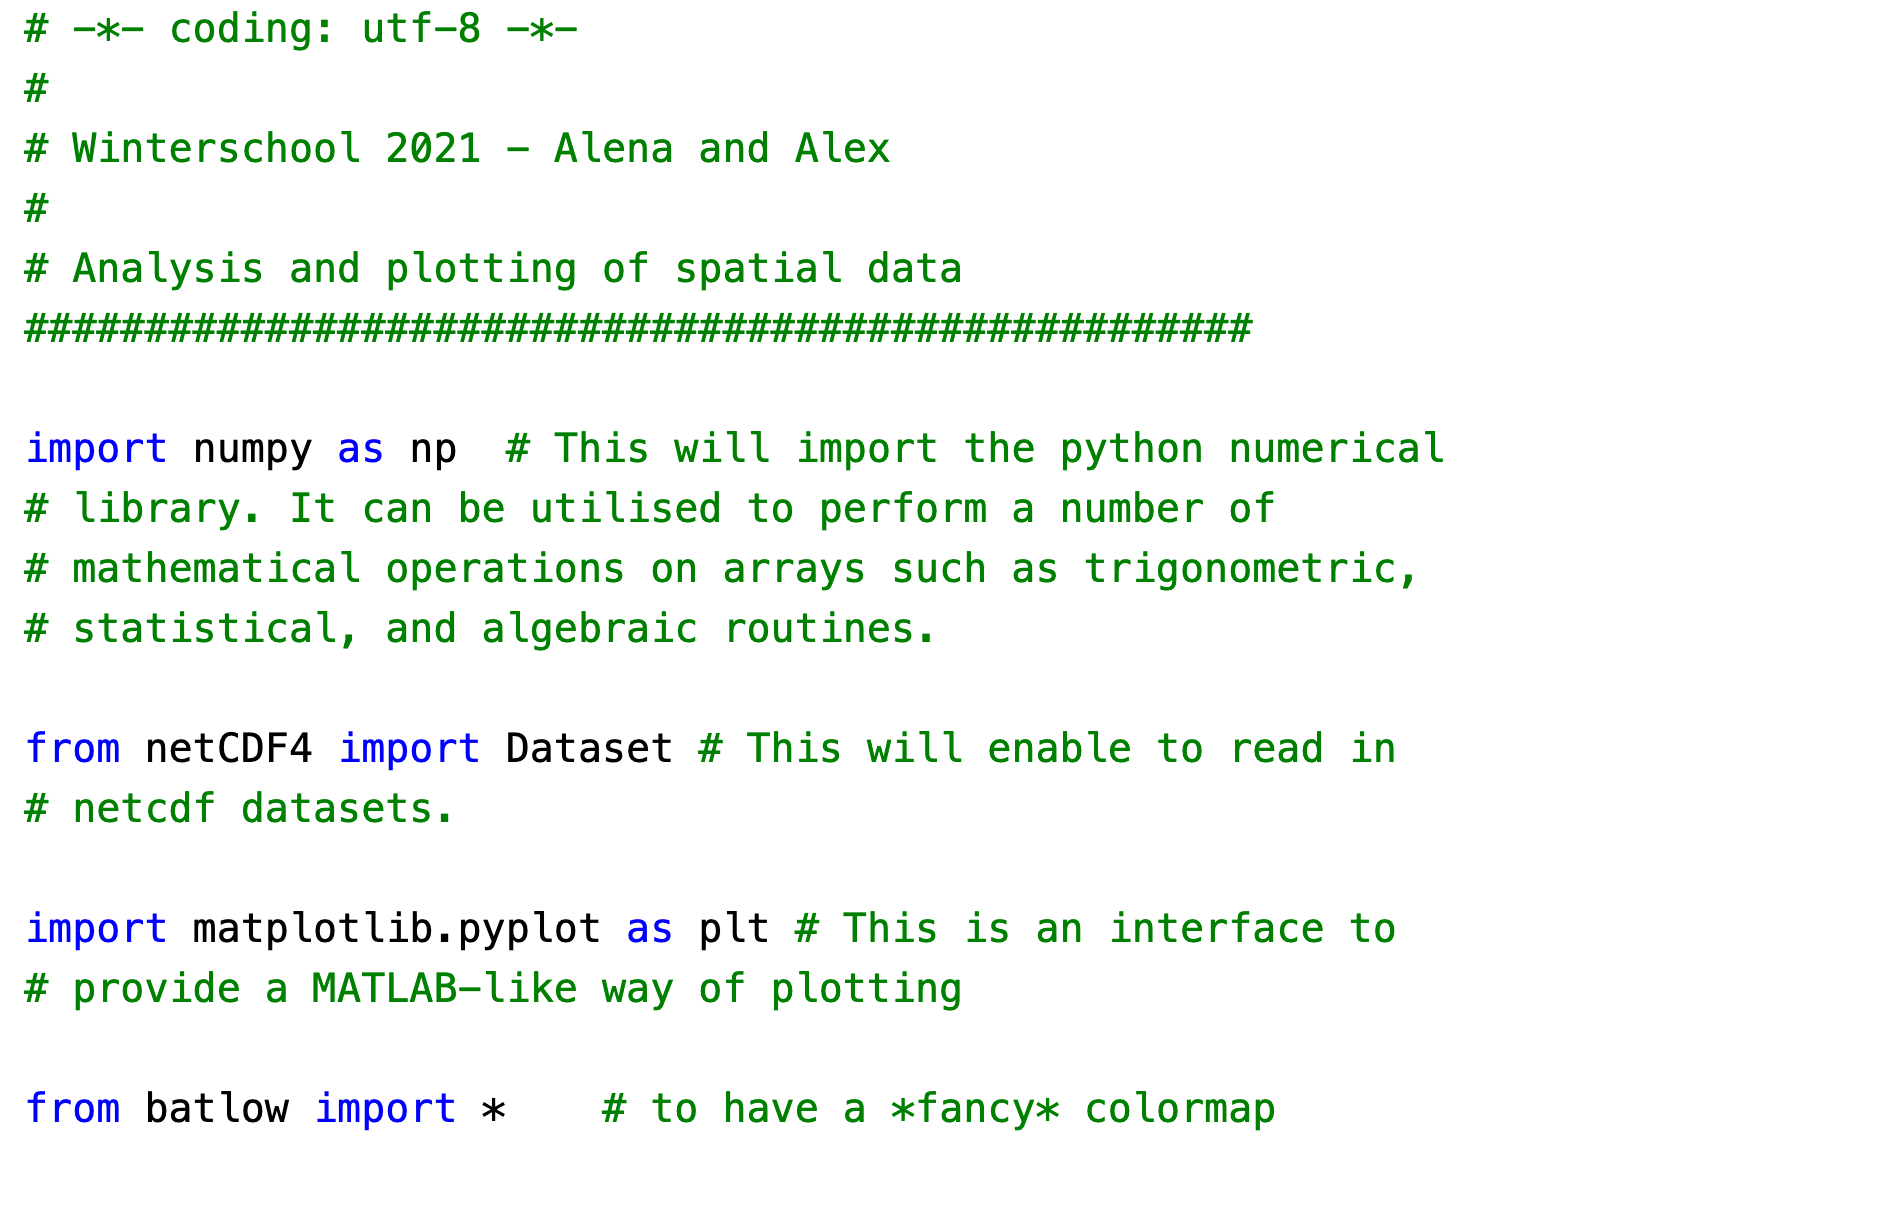
\includegraphics[scale=0.35]{images/Script1_step1.png}
\end{frame}
 
 
\begin{frame}{\textbf{3 |} Load into Python and visualise} 
    Let's import the netcdf dataset and get a sense of the dimensions:\\
        \vspace{0.5cm}
    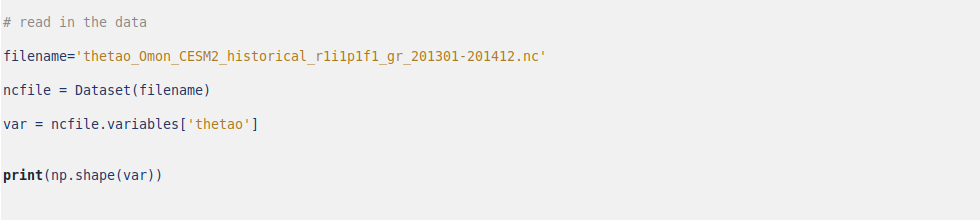
\includegraphics[scale=0.35]{images/Script1_step2.png}
        \vspace{2cm}
    (24, 33, 180, 360)
\end{frame}
 
 
\begin{frame}{\textbf{3 |} Load into Python and visualise} 
    Let's get the dimensions we want and plot the data:\\
        \vspace{0.5cm}
    here we want to look at the surface of the whole file
        \vspace{0.5cm}
    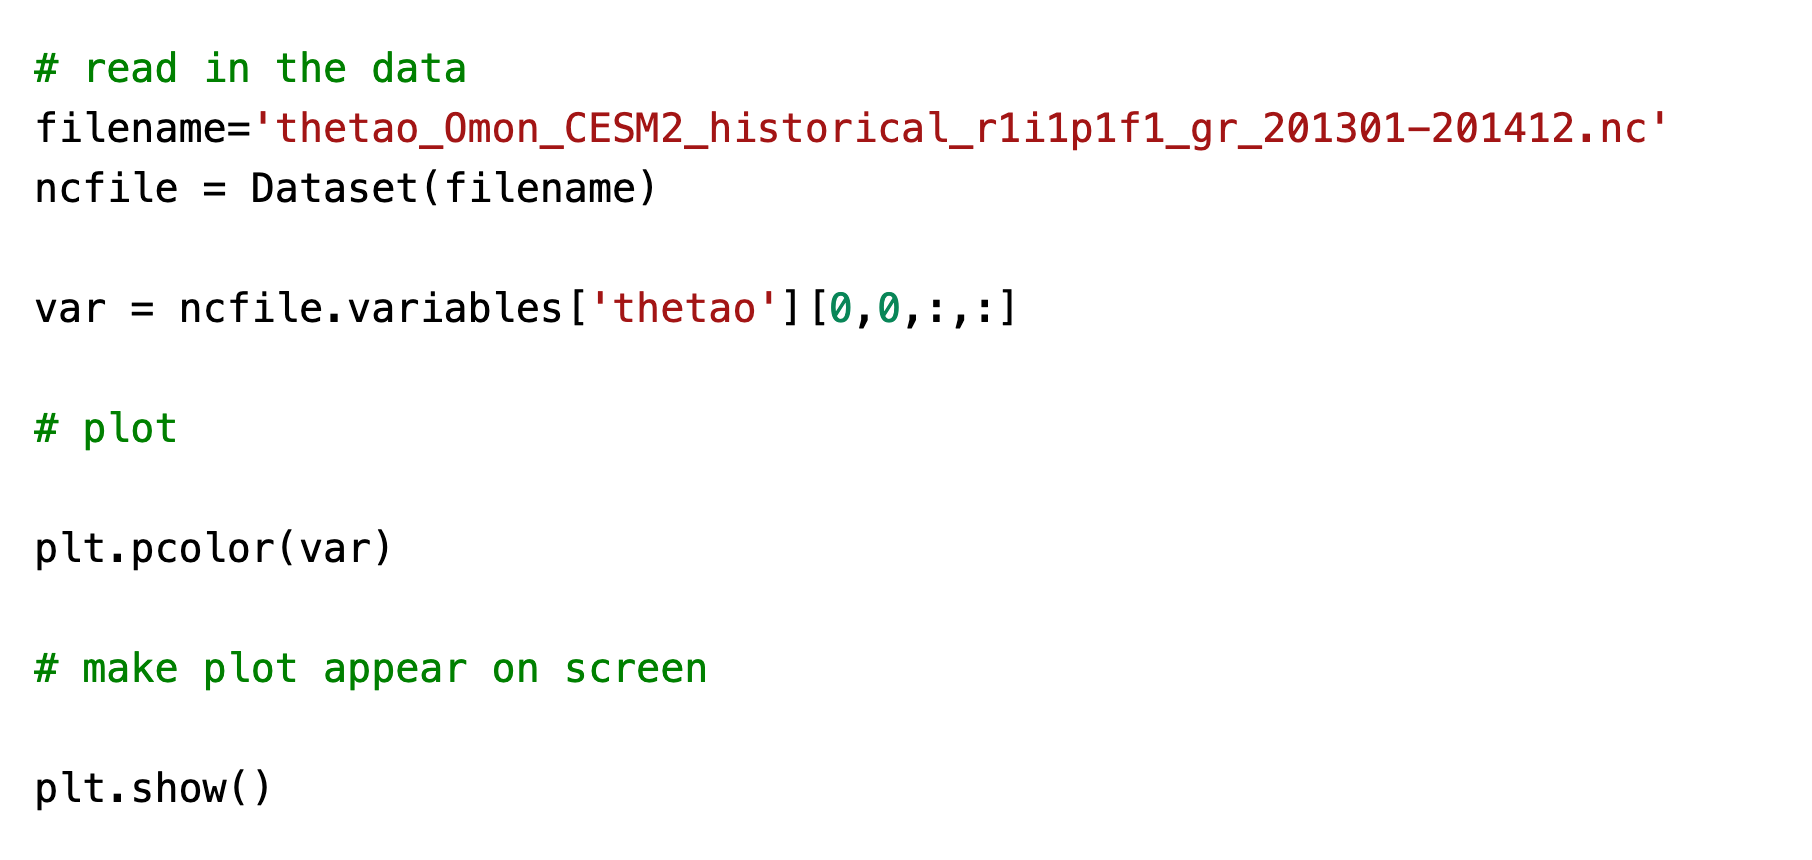
\includegraphics[scale=0.35]{images/Script1_step3.png}
\end{frame}
 
 
\begin{frame}{\textbf{3 |} Load into Python and visualise} 
    Let's get the dimensions we want and plot the data:\\
        \vspace{0.5cm}
    Here we want to look at the surface of the whole file
        \vspace{0.5cm}
    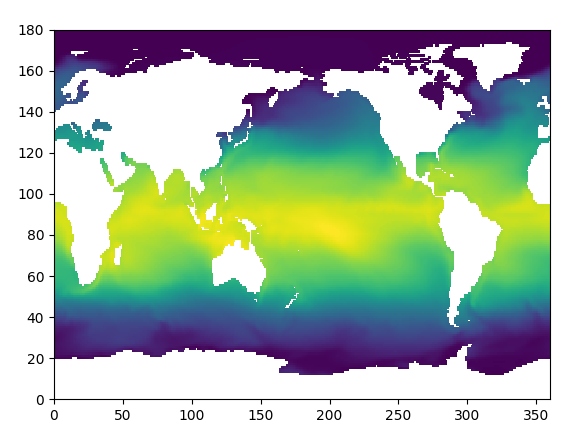
\includegraphics[scale=0.35]{images/script1_fig1.png}
\end{frame}
 
  
\begin{frame}{\textbf{3 |} Load into Python and visualise} 
    Let's add the latitude and longitude coordinates:\\
        \vspace{0.5cm}
    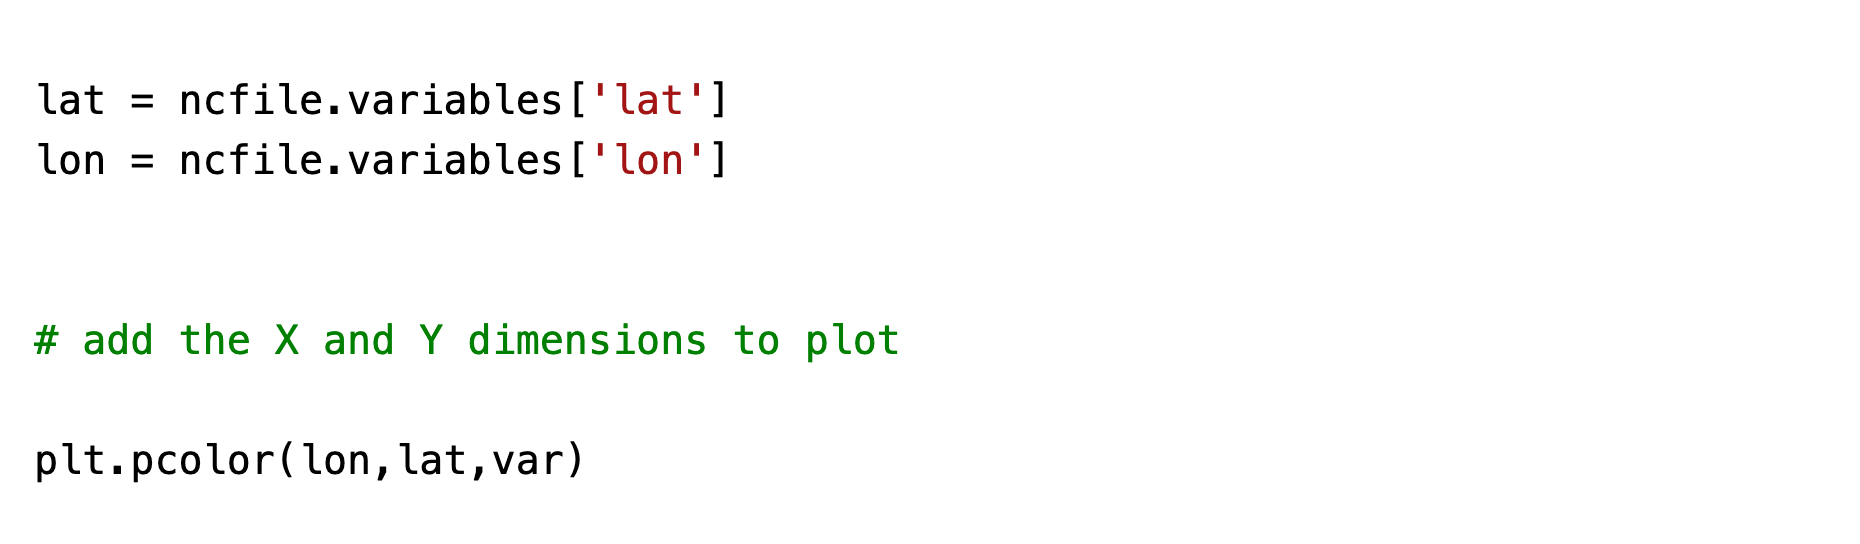
\includegraphics[scale=0.35]{images/Script1_step4.png}
\end{frame}
  
  
\begin{frame}{\textbf{3 |} Load into Python and visualise} 
    Let's add the latitude and longitude coordinates:\\
        \vspace{0.5cm}
    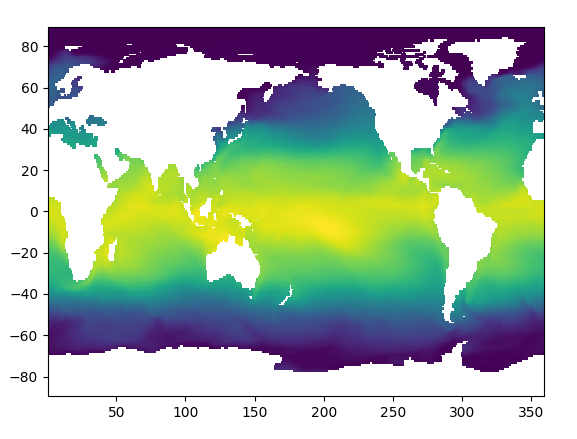
\includegraphics[scale=0.35]{images/Script1_fig2.png}
\end{frame}
 
 
\begin{frame}{\textbf{3 |} Load into Python and visualise} 
     Let's add a *fancy* colormap:\\
        \vspace{0.5cm}
    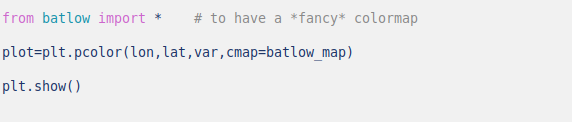
\includegraphics[scale=0.35]{images/Script1_step5.png}\\
        \vspace{0.5cm} This is based on \\
    
\includegraphics[scale=0.35]{images/Nature.png}\\
    (!! we need to add the batlow.py to the working directory)
\end{frame}
 
 
\begin{frame}{\textbf{3 |} Load into Python and visualise} 
    Let's add a *fancy* colormap:\\
        \vspace{0.5cm}
    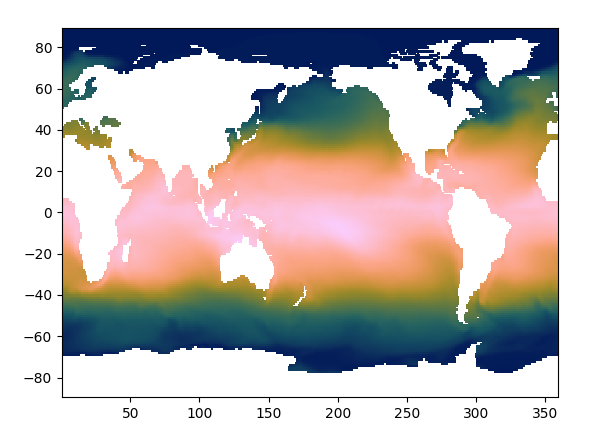
\includegraphics[scale=0.35]{images/Script1_fig3.png}
\end{frame}
 
 
\begin{frame}{\textbf{3 |} Load into Python and visualise} 
    Let's add a *fancy* colormap:\\
        \vspace{0.5cm}
    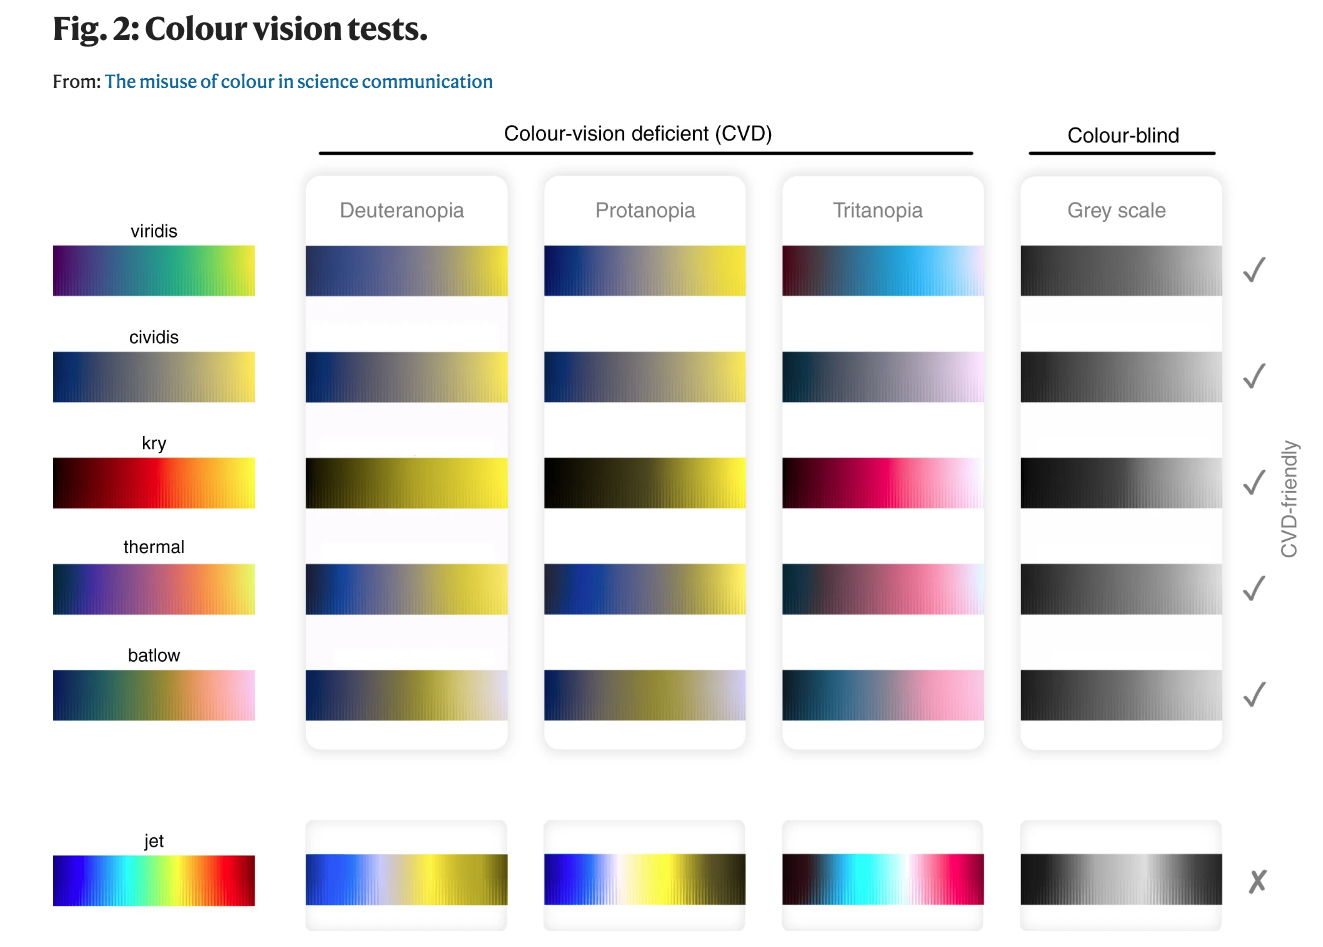
\includegraphics[scale=0.20]{images/Colormap_1.png}
\end{frame}
 
 
\begin{frame}{\textbf{3 |} Load into Python and visualise} 
    Let's add a *fancy* colormap:\\
        \vspace{0.5cm}
    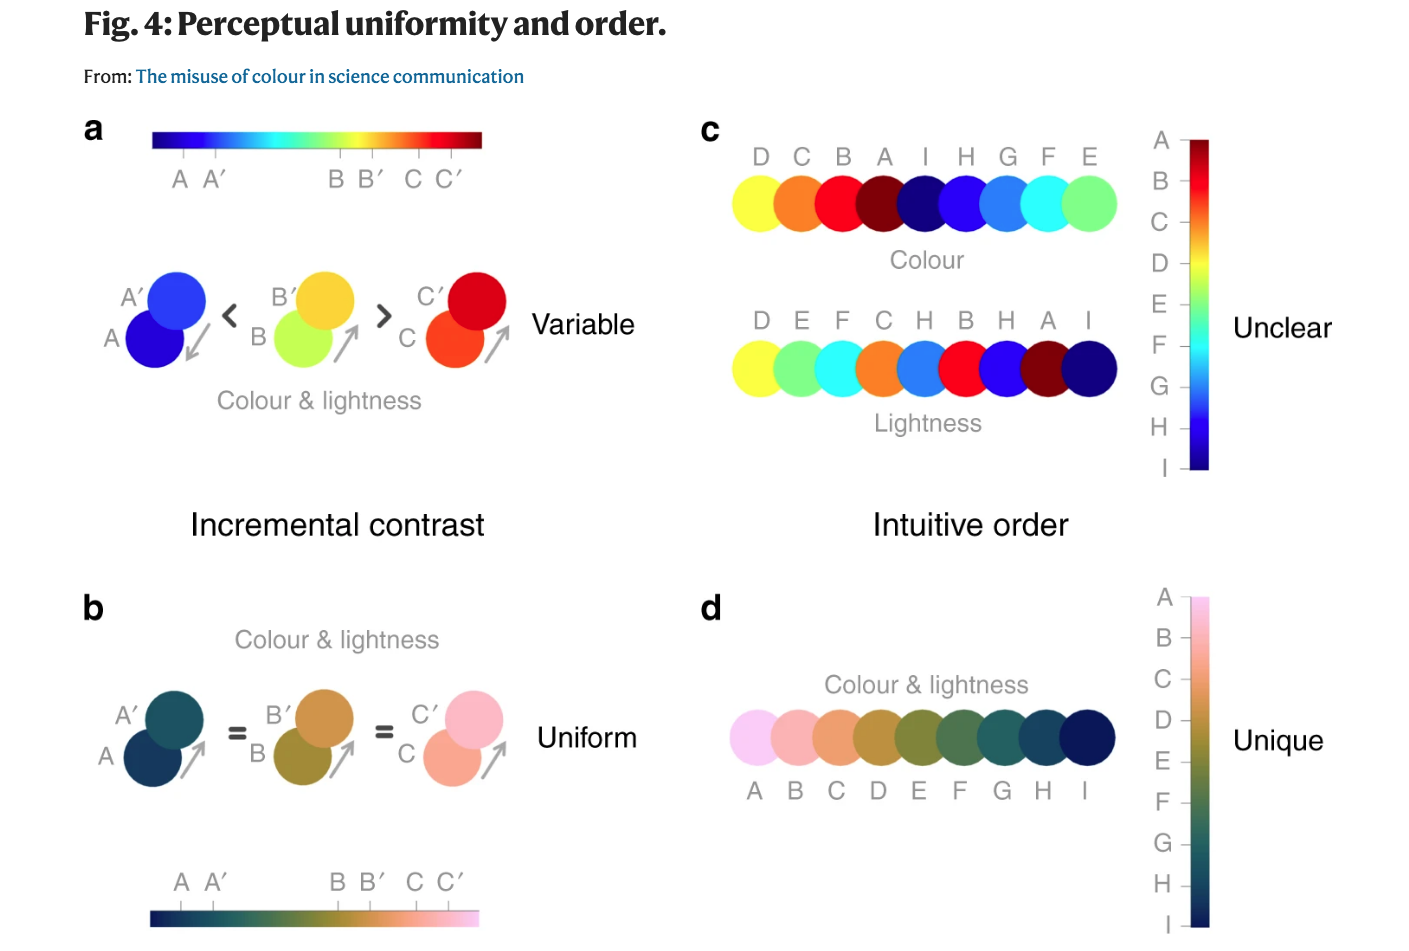
\includegraphics[scale=0.20]{images/Colormap_2.png}
\end{frame}
  
\begin{frame}{\textbf{3 |} Load into Python and visualise} 
    Let's add a *fancy* colormap:\\
        \vspace{0.5cm}
    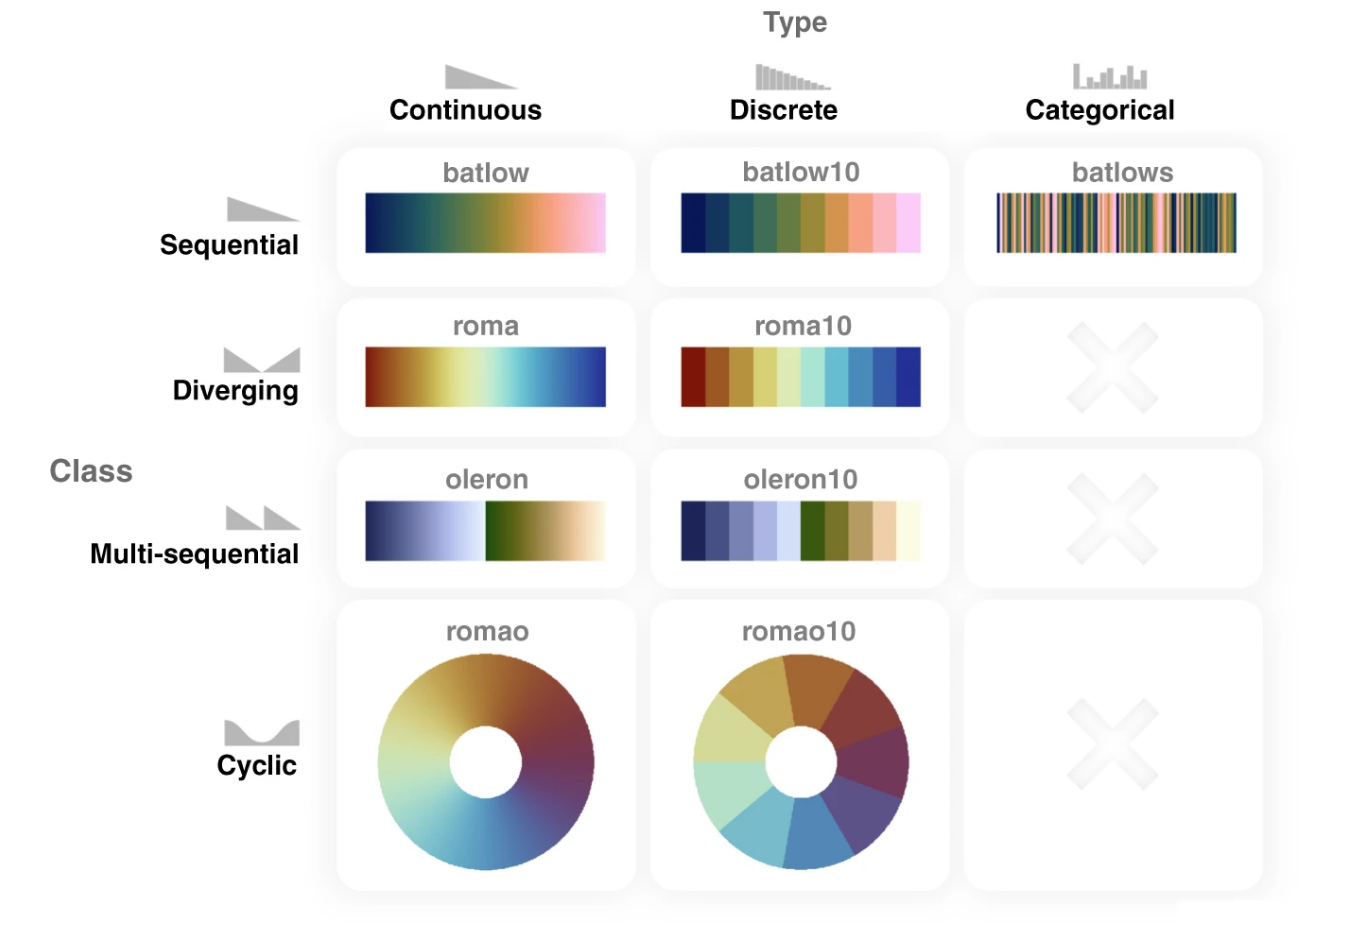
\includegraphics[scale=0.20]{images/Colormap_3.png}
\end{frame}
  
  
 
\begin{frame}{\textbf{3 |} Load into Python and visualise} 
    Let's add labels and a colorbar, but pay attention to the variable names and units!
        \vspace{0.5cm}
    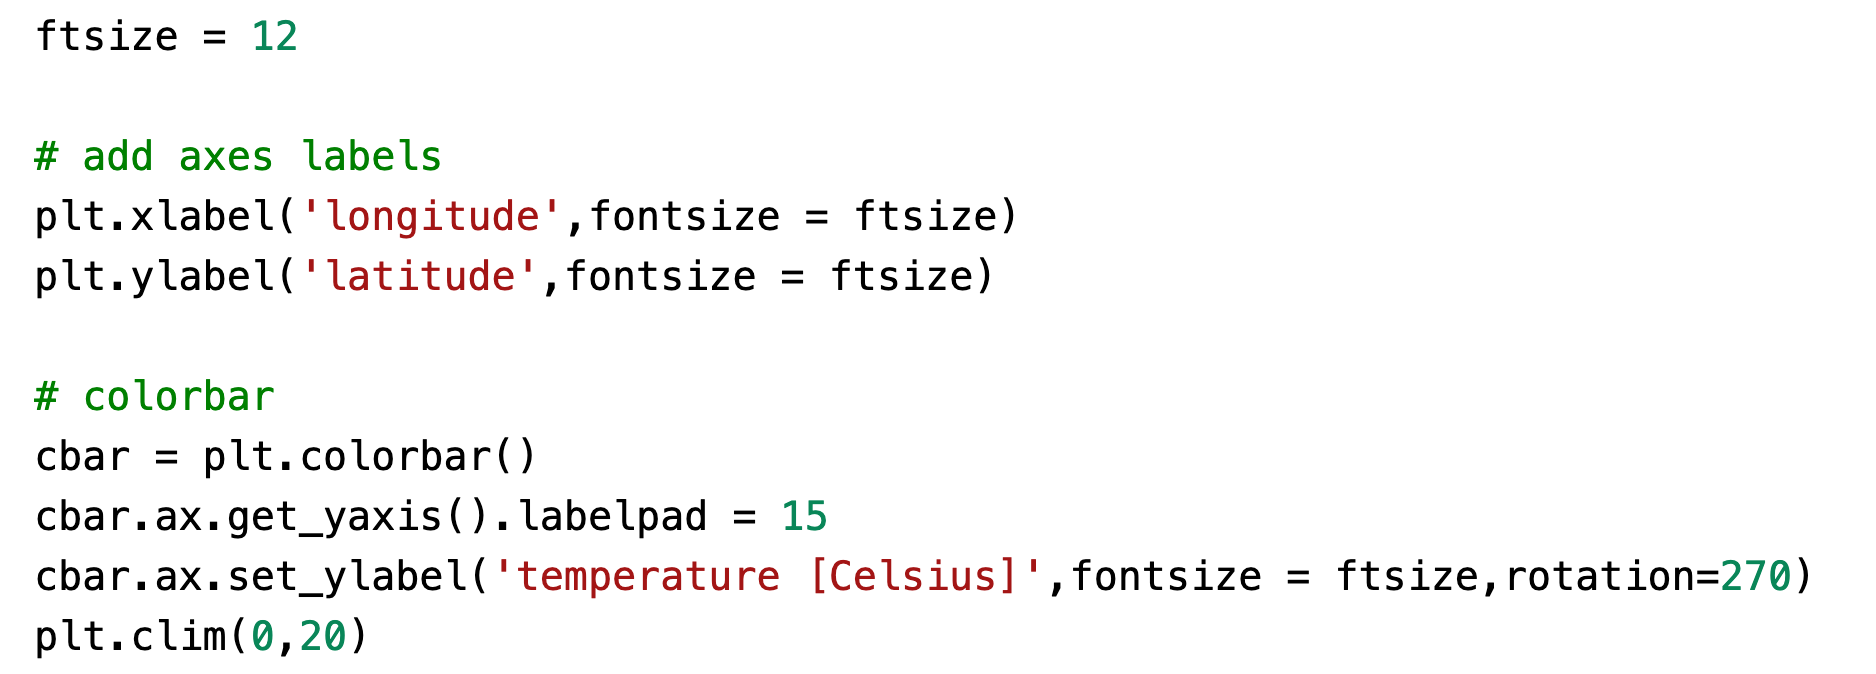
\includegraphics[scale=0.35]{images/Script1_step6.png}
\end{frame}
 
 
\begin{frame}{\textbf{3 |} Load into Python and visualise} 
    Let's add labels and a colorbar:\\
        \vspace{0.5cm}
    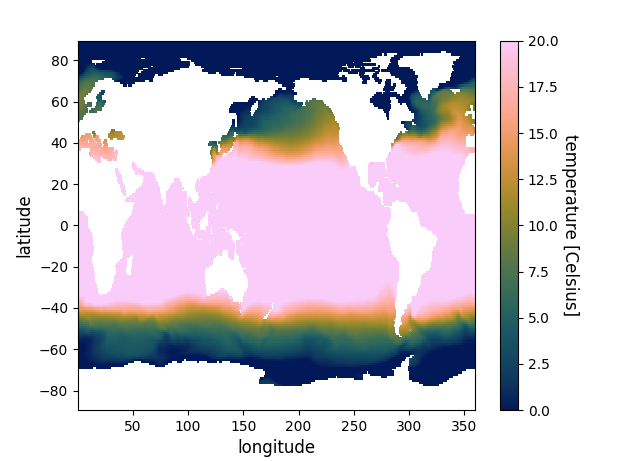
\includegraphics[scale=0.35]{images/Script1_fig4.png}
\end{frame}
 
 
\begin{frame}{\textbf{3 |} Load into Python and visualise} 
    And, if we wanted to mask out some data, we can use \textbf{cdo} as done previously, but also do it here:\\
        \vspace{0.3cm}
    To mask out a certain value:\\
        \vspace{0.5cm}
    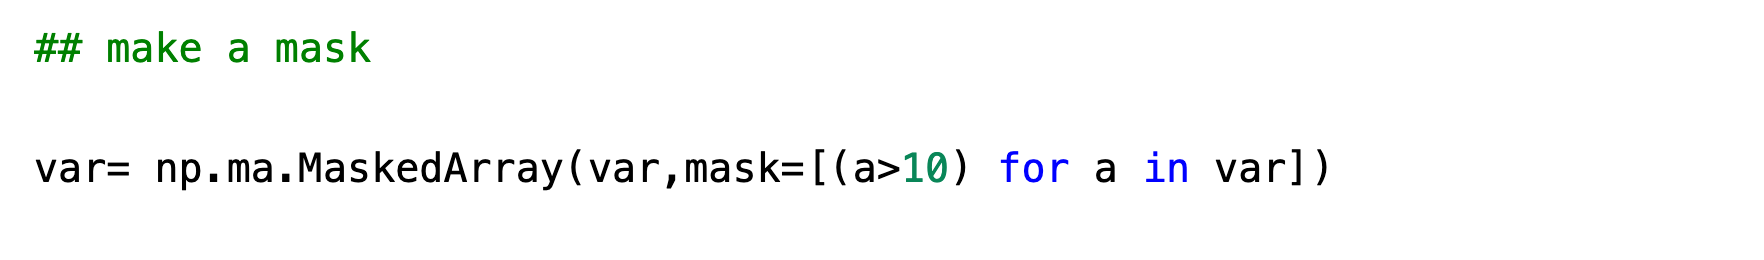
\includegraphics[scale=0.35]{images/Script1_step7.png}
        \vspace{0.5cm}
    and to mask an area based on lon/lat:
        \vspace{0.3cm}
    lon and lat are 1D variables, we need to make them 2D first
    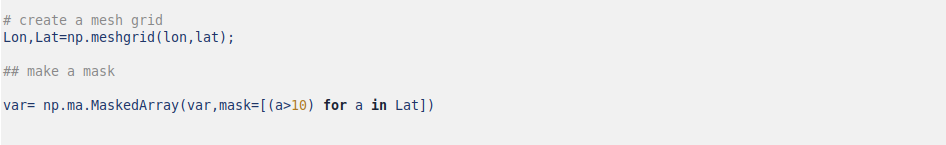
\includegraphics[scale=0.35]{images/Script1_step8.png}  
        \vspace{0.3cm}
\end{frame}
 
  
\begin{frame}{\textbf{3 |} Load into Python and visualise} 
    And, if we wanted to mask out some data, we can use \textbf{cdo} as done previously, but also do it here:\\
        \vspace{0.3cm}
    \begin{columns}
        \column[c]{6.5cm}
        To mask out a certain value:
            \vspace{0.5cm}
        \centering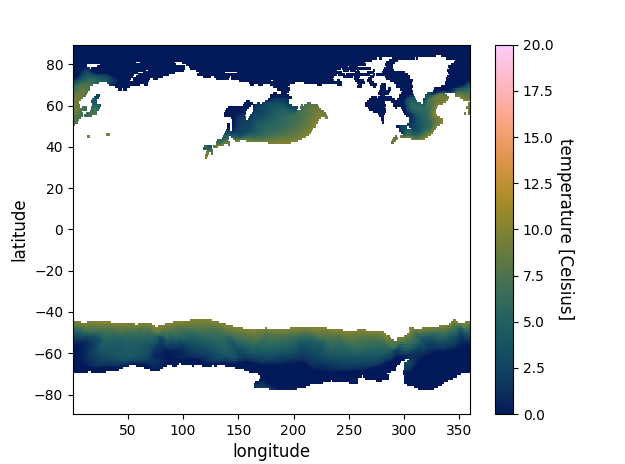
\includegraphics[scale=0.25]{images/Script1_fig5.png}
            \vspace{0.5cm}
        \column[c]{6.5cm}
        and to mask an area based on lon/lat:
            \vspace{0.3cm}
        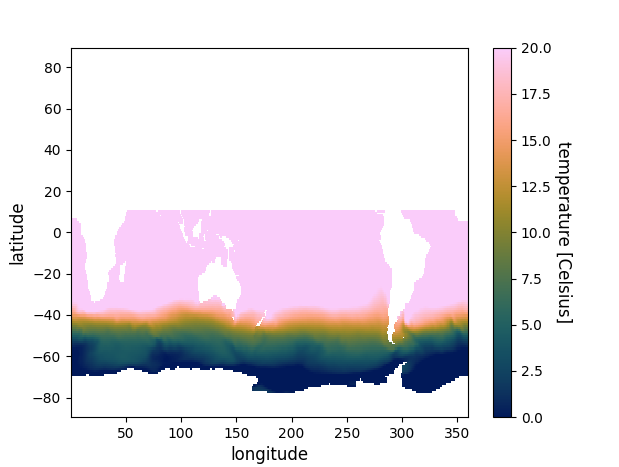
\includegraphics[scale=0.25]{images/Script1_fig6.png}
            \vspace{0.3cm}
    \end{columns}
\end{frame}

 
\begin{frame}{\textbf{3 |} Load into Python and visualise} 
    Now, we swap dimensions and plot along two of the 4 dimensions (lon versus time, depth versus time,...).\\
    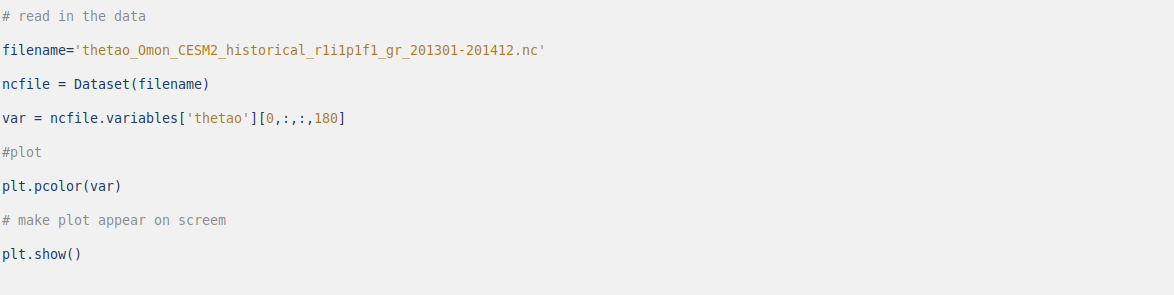
\includegraphics[scale=0.35]{images/Script1_step9.png}
    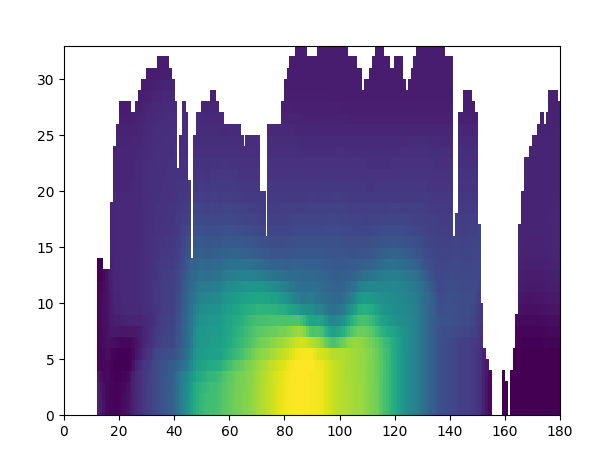
\includegraphics[scale=0.25]{images/Script1_fig7.png}
\end{frame}
 
  
\begin{frame}{\textbf{3 |} Load into Python and visualise} 
    To reverse the plot:\\
    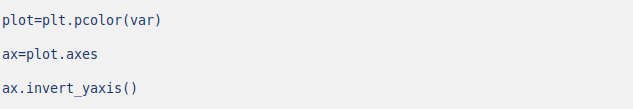
\includegraphics[scale=0.35]{images/Script1_step10.png}\\
    And add labels, colorbar,...
    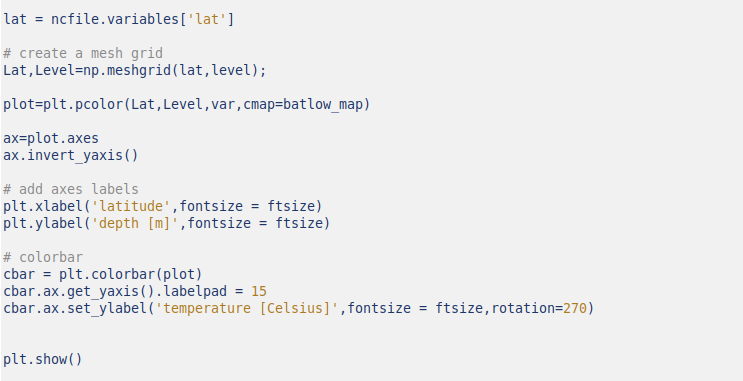
\includegraphics[scale=0.35]{images/Script1_step11.png}
\end{frame}
 
 
\begin{frame}{\textbf{3 |} Load into Python and visualise} 
    To reverse the plot:\\
    And add labels, colorbar,...
    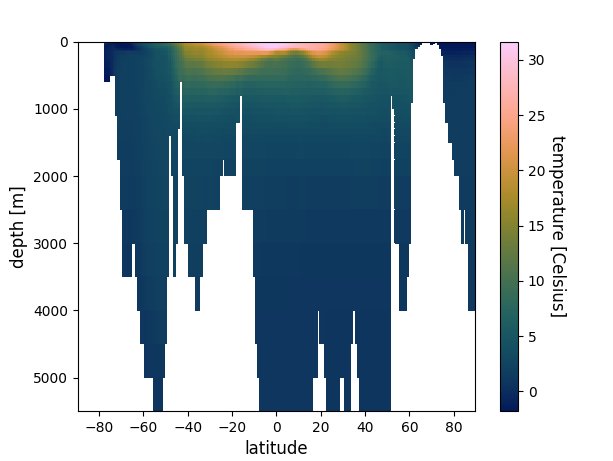
\includegraphics[scale=0.35]{images/script1_fig8.png}
\end{frame}


\begin{frame}{\textbf{3 |} Load into Python and visualise} 
    And finally add contour lines\\
    \includegraphics[scale=0.35]{images/script1_step12.png}\\
    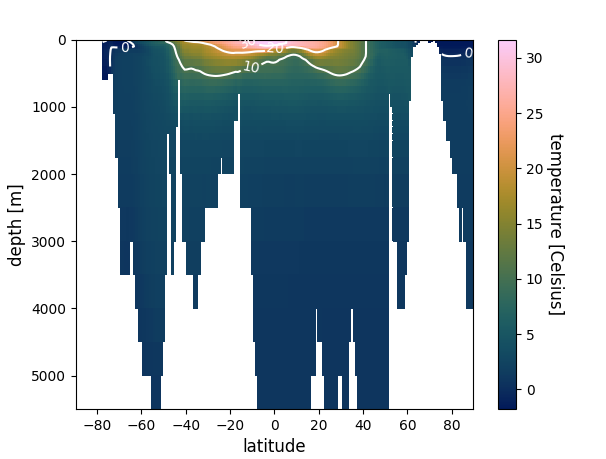
\includegraphics[scale=0.35]{images/script1_fig9.png}
\end{frame}


\begin{frame}{\textbf{3 |} Load into Python and visualise} 
    Let's plot one location over time, with depth: \\
    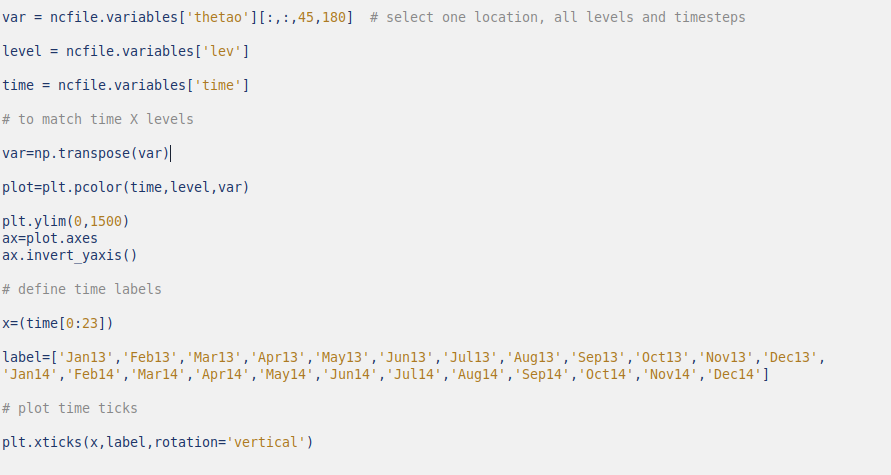
\includegraphics[scale=0.35]{images/Script1_step13.png}
\end{frame}


\begin{frame}{\textbf{3 |} Load into Python and visualise} 
    Let's plot one location over time, with depth: \\
    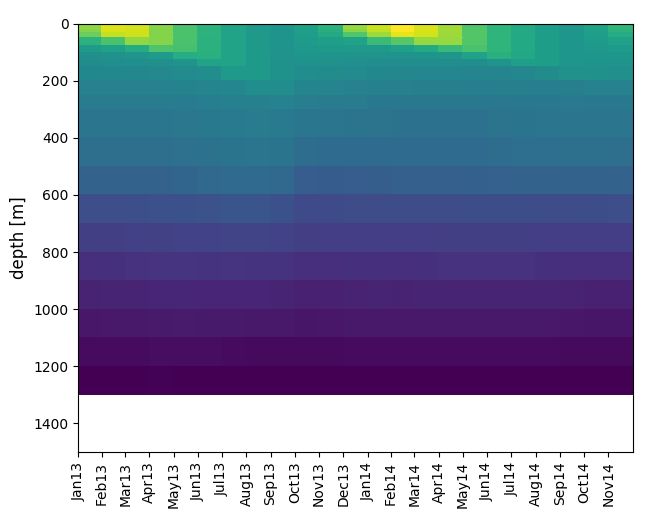
\includegraphics[scale=0.35]{images/script1_fig10.png}
\end{frame}


\begin{frame}{\textbf{3 |} Load into Python and visualise} 
    \begin{beamerboxesrounded}[lower=gray,shadow=true]{
        \begin{itemize}
            \item Try to find another location (different hemisphere or equator), or change the depth range on the y-axis.
            \item Do an horizontal section along the equator / 30S with depth values. Compare the extent of the mixed layers
        \end{itemize}}
    \end{beamerboxesrounded}
\end{frame} 

%*****************************************************************
% SEC4 |Make a publication figure
%*****************************************************************

\begin{frame}{\textbf{4 |} Make a publication figure} 
    Now that we have a pretty figure, let's start being fancy.\\
        \vspace{0.3cm}
    Mapping is the \textbf{second} step, not the first!\\
        \vspace{0.5cm}
    We will use the \href{https://scitools.org.uk/cartopy/docs/latest/}{\beamerbutton{cartopy}} package:\\
    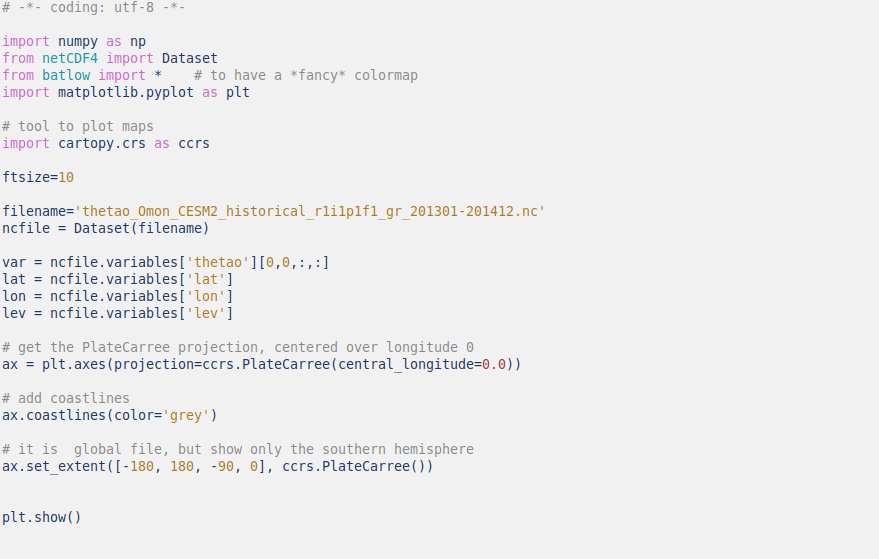
\includegraphics[scale=0.35]{images/Script2_step1.png}
\end{frame}
 

\begin{frame}{\textbf{4 |} Make a publication figure} 
    Now that we have a pretty figure, let's start being fancy.\\
        \vspace{0.3cm}
    Let's plot SST at the surface, over the whole domain with the 'Plate Carree" projection
        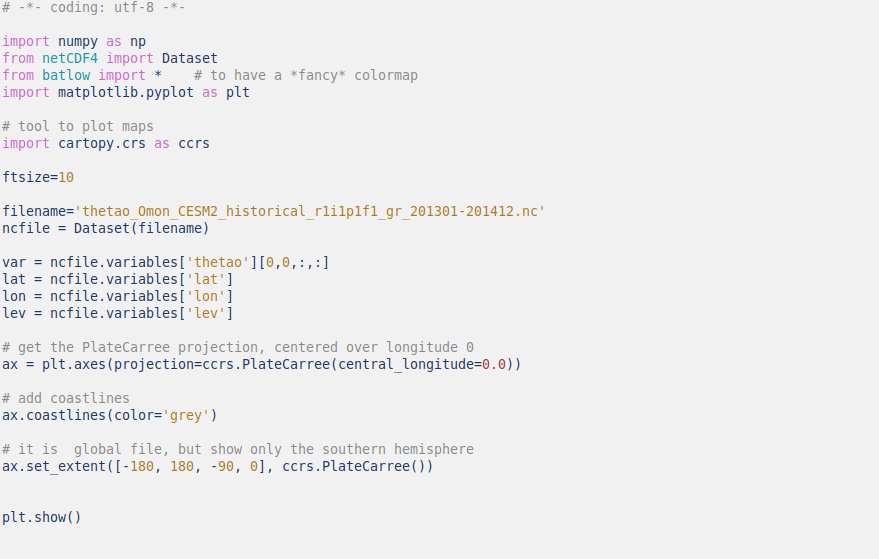
\includegraphics[scale=0.35]{images/Script2_step1.png}
\end{frame}
  
  
\begin{frame}{\textbf{4 |} Make a publication figure} 
    Now that we have a pretty figure, let's start being fancy.\\
        \vspace{0.5cm}
    Let's plot SST at the surface, over the whole domain with the 'Plate Carree" projection
    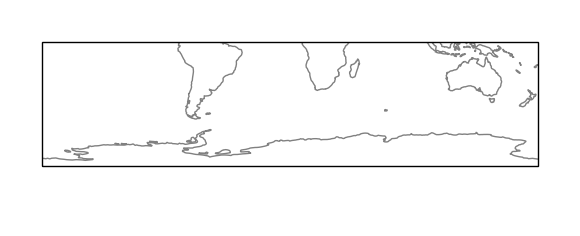
\includegraphics[scale=0.35]{images/script2_fig1.png}
\end{frame}


\begin{frame}{\textbf{4 |} Make a publication figure} 
    Now that we have a pretty figure, let's start being fancy.\\
        \vspace{0.5cm}
    Let's fill in the variable, but lat and lon have to be  2D (use meshgrid)
    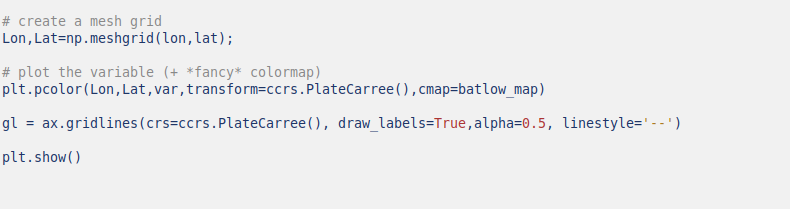
\includegraphics[scale=0.35]{images/Script2_step2.png}
\end{frame}


\begin{frame}{\textbf{4 |} Make a publication figure} 
    Now that we have a pretty figure, let's start being fancy.\\
        \vspace{0.5cm}
    Let's fill in the variable, but lat and lon have to be 2D (use meshgrid)
    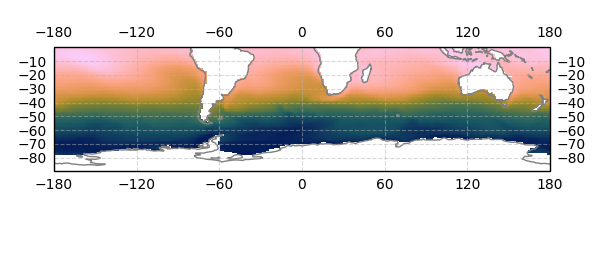
\includegraphics[scale=0.45]{images/script2_fig2.png}
\end{frame}
 
 
\begin{frame}{\textbf{4 |} Make a publication figure} 
    Now that we have a pretty figure, let's start being fancy.\\
        \vspace{0.5cm}
    Format the axes 
    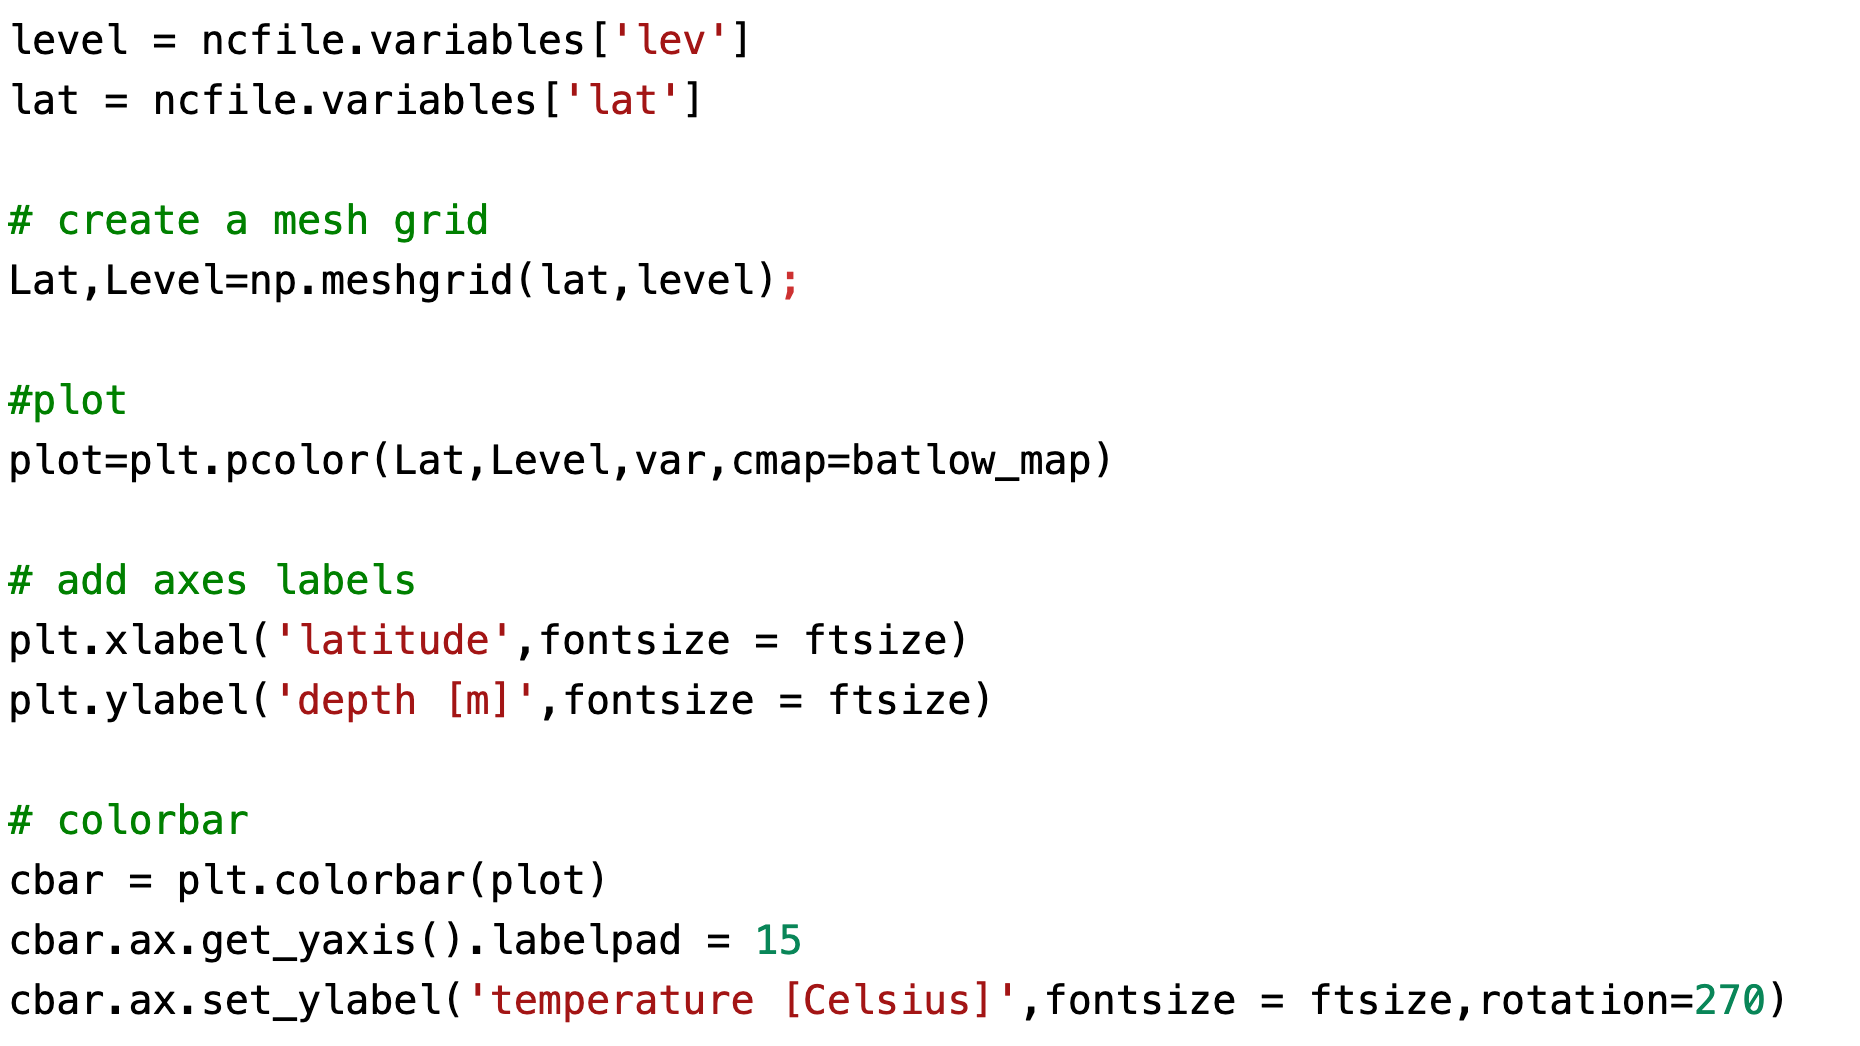
\includegraphics[scale=0.35]{images/Script2_step3.png}
\end{frame}


\begin{frame}{\textbf{4 |} Make a publication figure} 
    Now that we have a pretty figure, let's start being fancy.\\
        \vspace{0.5cm}
    Format the axes \\
    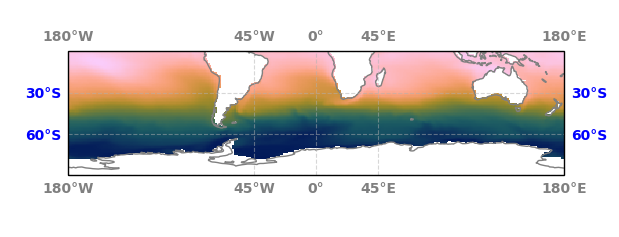
\includegraphics[scale=0.45]{images/script2_fig3.png}
\end{frame}


\begin{frame}{\textbf{4 |} Make a publication figure} 
    Now that we have a pretty figure, let's start being fancy.\\
        \vspace{0.5cm}
    Imagine we have a CTD station (at 60W 40S and 4500 m depth (30th level)) and we want to indicate it on the map\\
    + add the colorbar\\
    \includegraphics[scale=0.35]{images/Script2_step4.png}
\end{frame}


\begin{frame}{\textbf{4 |} Make a publication figure} 
    Now that we have a pretty figure, let's start being fancy.\\
        \vspace{0.5cm}
    Imagine we have a CTD station and we want to indicate it on the map\\
    + add the colorbar\\
        \vspace{0.5cm}
    \includegraphics[scale=0.45]{images/script2_fig4.png}
\end{frame}


\begin{frame}{\textbf{4 |} Make a publication figure} 
    What if we want to compare two datasets, which are not on the same grid? \\
        \vspace{0.5cm}
    Re-Mapping is the answer !\\
        \vspace{0.5cm}
    We can do it in \textbf{cdo}: \\
    \textit{cdo remapbil ...} will use bilinear interpolation to remap one grid ont another \\
    (! create a grid description file using \textit{cdo griddes} beforehand)\\
        \vspace{0.5cm}
    Get the grid description of the file you want to remap \textbf{onto}: (here, ERA5)\\
    \textcolor{black}{cdo griddes SST\_ERA5\_201301.nc > grid\_era5.txt}\\
    \includegraphics[scale=0.35]{images/Script3_step1.png}
\end{frame}
  
  
 \begin{frame}{\textbf{4 |} Make a publication figure} 
    What if we want to compare two datasets, which are not on the same grid? \\
        \vspace{0.3cm}
    Re-Mapping is the answer !
        \vspace{0.3cm}
    We can do it in cdo: \\
    \textcolor{black}{cdo remapbil,grid\_era5.txt thetao\_Omon\_CESM2\_historical\_r1i1p1f1\_gr\_201301-201412.nc theta\_remapped.nc}\\
    (check the nc file)\\
        \vspace{0.5cm}
    To subtract one from the other, the two files have to have the 'same variable' (name):\\
        \vspace{0.3cm} 
    \textcolor{black}{cdo chname,thetao,sst theta\_remapped.nc theta\_remapped\_sst.nc} \\
    (check the nc file)\\
        \vspace{0.3cm} 
    \textcolor{black}{cdo sub SST\_ERA5\_201301.nc theta\_remapped\_sst.nc diff\_era5\_theta.nc} \\
    (check the nc file, and play with the colorbar, range,...)
\end{frame}

  
\begin{frame}{\textbf{4 |} Make a publication figure} 
    Now, let's do the same in Python !\\
        \vspace{0.5cm} 
    We will use the \textbf{griddata package}\\
    \includegraphics[scale=0.35]{images/Script5_step1.png}
\end{frame}
  
  
\begin{frame}{\textbf{4 |} Make a publication figure} 
    We will use the \textbf{griddata package}\\
    \includegraphics[scale=0.30]{images/script5_fig1.png}
\end{frame}

\begin{frame}{\textbf{4 |} Make a publication figure} 
    We will use the \textbf{griddata package}\\
        \vspace{0.3cm} 
    And it needs the data to be formatted in a specific way:
    \includegraphics[scale=0.35]{images/Script5_step2.png}
\end{frame}


\begin{frame}{\textbf{4 |} Make a publication figure} 
    We will use the \textbf{griddata package}\\
        \vspace{0.3cm} 
    And it needs the data to be formatted in a specific way:
    \includegraphics[scale=0.35]{images/Script5_step3.png}
\end{frame}


\begin{frame}{\textbf{4 |} Make a publication figure} 
    We will use the \textbf{griddata package}\\
        \vspace{0.3cm} 
    Let's make 3 subplots in the figure: \\
    \begin{itemize}
        \item the ERA5 data
        \item the CMIP regridded data
    \end{itemize}
    \includegraphics[scale=0.35]{images/Script5_step4.png}
\end{frame}

\begin{frame}{\textbf{4 |} Make a publication figure} 
    We will use the \textbf{griddata package}\\
        \vspace{0.3cm} 
    Let's make 3 subplots in the figure: \\
    \begin{itemize}
        \item the ERA5 data
        \item the CMIP regridded data
    \end{itemize}
    \includegraphics[scale=0.30]{images/script5_fig1.png}
\end{frame}


\begin{frame}{\textbf{4 |} Make a publication figure} 
    We will use the \textbf{griddata package}\\
        \vspace{0.3cm} 
    Let's make 3 subplots in the figure: 
    \begin{itemize}
        \item the ERA5 data
        \item the CMIP regridded data
        \item the difference between the two
    \end{itemize}
    \includegraphics[scale=0.35]{images/Script5_step5.png}
\end{frame}

\begin{frame}{\textbf{4 |} Make a publication figure} 
    We will use the \textbf{griddata package}\\
        \vspace{0.3cm} 
    Let's make 3 subplots in the figure: \\
    \begin{itemize}
        \item the ERA5 data
        \item the CMIP regridded data
        \item the difference between the two
    \end{itemize}
    \includegraphics[scale=0.25]{images/script5_fig2.png}
\end{frame}

\begin{frame}{\textbf{4 |} Make a publication figure} 
    We will use the \textbf{griddata package}\\
        \vspace{0.3cm} 
    Add the colorbars : \\
    \begin{itemize}
        \item batlow, but same limits
        \item batlow, but same limits
    \end{itemize}
    Hint: we can print out the min and max values of our variables :
    \includegraphics[scale=0.35]{images/hint.png}\\
    \includegraphics[scale=0.35]{images/Script5_step7.png}
\end{frame}


\begin{frame}{\textbf{4 |} Make a publication figure} 
    We will use the \textbf{griddata package}\\
        \vspace{0.3cm} 
    Add the colorbars : \\
    \begin{itemize}
        \item batlow, but same limits
        \item batlow, but same limits
        \item red-blue and centered around 0 (the vik colorbar)! 
    \end{itemize}
    \includegraphics[scale=0.35]{images/script5_step6.png}
\end{frame}


\begin{frame}{\textbf{4 |} Make a publication figure} 
    We will use the \textbf{griddata package}\\
        \vspace{0.3cm} 
    \begin{itemize}
        \item batlow, but same limits
        \item batlow, but same limits
        \item red-blue and centered around 0 (the vik colorbar)! 
    \end{itemize}
    \includegraphics[scale=0.35]{images/Script5_step8.png}
\end{frame}


\begin{frame}{\textbf{4 |} Make a publication figure} 
    We will use the \textbf{griddata package}\\
        \vspace{0.3cm} 
    Add the colorbars : \\
    \begin{columns}
        \column[c]{6.5cm}
            \includegraphics[width=6cm]{images/script5_fig4.png}
        \column[c]{6.5cm}
            \begin{beamerboxesrounded}[lower=gray,shadow=true]{
                Our figure will \textbf{not} look like this,\\
                find out why and fix it!}
            \end{beamerboxesrounded}
    \end{columns}
\end{frame}


\begin{frame}{\textbf{4 |} Make a publication figure} 
    We will use the \textbf{griddata package}\\
        \vspace{0.3cm} 
    Finally, set the layout and save the figure \\
    \includegraphics[scale=0.35]{images/Script5_step9.png}
\end{frame}


\begin{frame}{\textbf{4 |} Make a publication figure} 
    \begin{beamerboxesrounded}[lower=gray,shadow=true]{
        Let's do the same as for the final \textit{cdo} command, but in a python script:\\
            \vspace{0.5cm}
        Compare two cross sections of the mean June sst value over the dateline. \\
            \vspace{0.5cm}
        using the two thetao files (201301-201412 and 185001-185112).\\
            \vspace{0.5cm}
        and using the red-blue colormap, invert the y scale and make the colorbar symmetrical around 0\\
            \vspace{2cm}}
    \end{beamerboxesrounded}
\end{frame}


\begin{frame}{\textbf{4 |} Make a publication figure} 
    Let's do the same as for the final \textbf{cdo} command, but in a python script:\\
        \vspace{0.5cm}
    \includegraphics[scale=0.20]{images/ERA5_difference_2013_1850_june.png}\\
    And as a final check, load your cdo final result and compare to the output of this script!
\end{frame}


\begin{frame}{\textbf{4 |} Make a publication figure} 
    Let's do the same as for the final \textbf{cdo} command, but in a python script:\\
        \vspace{0.5cm}
    \includegraphics[scale=0.20]{images/difference_cdo_python.png}\\
    And as a final check, load your cdo final result and compare to the output of this script!
\end{frame}

%%%%%%%%%%%%%%%%%%%%%%%% END CONTENT %%%%%%%%%%%%%%%%%%%%%%
